%%% Hlavní soubor. Zde se definují základní parametry a odkazuje se na ostatní části. %%%

%% Verze pro jednostranný tisk:
% Okraje: levý 40mm, pravý 25mm, horní a dolní 25mm
% (ale pozor, LaTeX si sám přidává 1in)
\documentclass[12pt,a4paper]{report}
\setlength\textwidth{145mm}
\setlength\textheight{247mm}
\setlength\oddsidemargin{15mm}
\setlength\evensidemargin{15mm}
\setlength\topmargin{0mm}
\setlength\headsep{0mm}
\setlength\headheight{0mm}
% \openright zařídí, aby následující text začínal na pravé straně knihy
\let\openright=\clearpage

%% Pokud tiskneme oboustranně:
% \documentclass[12pt,a4paper,twoside,openright]{report}
% \setlength\textwidth{145mm}
% \setlength\textheight{247mm}
% \setlength\oddsidemargin{14.2mm}
% \setlength\evensidemargin{0mm}
% \setlength\topmargin{0mm}
% \setlength\headsep{0mm}
% \setlength\headheight{0mm}
% \let\openright=\cleardoublepage

%% Vytváříme PDF/A-2u
\usepackage[a-2u]{pdfx}

%% Přepneme na českou sazbu a fonty Latin Modern
\usepackage[czech]{babel}
\usepackage{lmodern}
\usepackage[T1]{fontenc}
\usepackage{textcomp}

%% Použité kódování znaků: obvykle latin2, cp1250 nebo utf8:
\usepackage[utf8]{inputenc}

%%% Další užitečné balíčky (jsou součástí běžných distribucí LaTeXu)
\usepackage{amsmath}        % rozšíření pro sazbu matematiky
\usepackage{amsfonts}       % matematické fonty
\usepackage{amsthm}         % sazba vět, definic apod.
\usepackage{bbding}         % balíček s nejrůznějšími symboly
			    % (čtverečky, hvězdičky, tužtičky, nůžtičky, ...)
\usepackage{bm}             % tučné symboly (příkaz \bm)
\usepackage{graphicx}       % vkládání obrázků
\usepackage{fancyvrb}       % vylepšené prostředí pro strojové písmo
\usepackage{indentfirst}    % zavede odsazení 1. odstavce kapitoly
\usepackage{natbib}         % zajištuje možnost odkazovat na literaturu
			    % stylem AUTOR (ROK), resp. AUTOR [ČÍSLO]
\usepackage[nottoc]{tocbibind} % zajistí přidání seznamu literatury,
                            % obrázků a tabulek do obsahu
\usepackage{icomma}         % inteligetní čárka v matematickém módu
\usepackage{dcolumn}        % lepší zarovnání sloupců v tabulkách
\usepackage{booktabs}       % lepší vodorovné linky v tabulkách
\usepackage{paralist}       % lepší enumerate a itemize
\usepackage{xcolor}         % barevná sazba
\usepackage{hyperref}       % odkazy

\usepackage{svg}
%\svgsetup{inkscapelatex=false}
\usepackage{tcolorbox}
\usepackage{float}
\usepackage{enumitem,amssymb}
% List with square bullets
\newlist{todolist}{itemize}{2}
\setlist[todolist]{label=$\square$}

%%% Údaje o práci

% Název práce v jazyce práce (přesně podle zadání)
\def\NazevPrace{Platforma pro monitorování mentálního zdraví}

% Název práce v angličtině
\def\NazevPraceEN{Mental health monitoring platform}

% Jméno autora
\def\AutorPrace{Patrik Trefil}

% Rok odevzdání
\def\RokOdevzdani{2023}

% Název katedry nebo ústavu, kde byla práce oficiálně zadána
% (dle Organizační struktury MFF UK, případně plný název pracoviště mimo MFF)
\def\Katedra{Katedra softwarového inženýrství (204. • 32-KSI)}
\def\KatedraEN{Department of Software Engineering}

% Jedná se o katedru (department) nebo o ústav (institute)?
\def\TypPracoviste{Katedra softwarového inženýrství (204. • 32-KSI)}
\def\TypPracovisteEN{Department of Software Engineering}

% Vedoucí práce: Jméno a příjmení s~tituly
\def\Vedouci{Mgr. Petr Škoda, Ph.D.}

% Pracoviště vedoucího (opět dle Organizační struktury MFF)
\def\KatedraVedouciho{Katedra softwarového inženýrství (204. • 32-KSI)}
\def\KatedraVedoucihoEN{Department of Software Engineering}

% Studijní program a obor
\def\StudijniProgram{Informatika (B0613A140006)}
\def\StudijniObor{IPP2 (0613RA1400060006)}

% Nepovinné poděkování (vedoucímu práce, konzultantovi, tomu, kdo
% zapůjčil software, literaturu apod.)
% TODO: doplnit poděkování
\def\Podekovani{%
Poděkování.
}

% Abstrakt (doporučený rozsah cca 80-200 slov; nejedná se o zadání práce)
% TODO: Doplnit abstrakt
\def\Abstrakt{%
Abstrakt.
}
% TODO: Doplnit abstrakt v angličtině
\def\AbstraktEN{%
Abstract.
}

% 3 až 5 klíčových slov (doporučeno), každé uzavřeno ve složených závorkách
\def\KlicovaSlova{%
{vývoj software}, {webová aplikace}, {formuláře}
}
\def\KlicovaSlovaEN{%
{software development}, {web application}, {forms}
}

%% Balíček hyperref, kterým jdou vyrábět klikací odkazy v PDF,
%% ale hlavně ho používáme k uložení metadat do PDF (včetně obsahu).
%% Většinu nastavítek přednastaví balíček pdfx.
\hypersetup{unicode}
\hypersetup{breaklinks=true}

%% Definice různých užitečných maker (viz popis uvnitř souboru)
%%% Tento soubor obsahuje definice různých užitečných maker a prostředí %%%
%%% Další makra připisujte sem, ať nepřekáží v ostatních souborech.     %%%

%%% Drobné úpravy stylu

% Tato makra přesvědčují mírně ošklivým trikem LaTeX, aby hlavičky kapitol
% sázel příčetněji a nevynechával nad nimi spoustu místa. Směle ignorujte.
\makeatletter
\def\@makechapterhead#1{
  {\parindent \z@ \raggedright \normalfont
   \Huge\bfseries \thechapter. #1
   \par\nobreak
   \vskip 20\p@
}}
\def\@makeschapterhead#1{
  {\parindent \z@ \raggedright \normalfont
   \Huge\bfseries #1
   \par\nobreak
   \vskip 20\p@
}}
\makeatother

% Toto makro definuje kapitolu, která není očíslovaná, ale je uvedena v obsahu.
\def\chapwithtoc#1{
\chapter*{#1}
\addcontentsline{toc}{chapter}{#1}
}

% Trochu volnější nastavení dělení slov, než je default.
\lefthyphenmin=2
\righthyphenmin=2

% Zapne černé "slimáky" na koncích řádků, které přetekly, abychom si
% jich lépe všimli.
\overfullrule=1mm

%%% Makra pro definice, věty, tvrzení, příklady, ... (vyžaduje baliček amsthm)

\theoremstyle{plain}
\newtheorem{veta}{Věta}
\newtheorem{lemma}[veta]{Lemma}
\newtheorem{tvrz}[veta]{Tvrzení}

\theoremstyle{plain}
\newtheorem{definice}{Definice}

\theoremstyle{remark}
\newtheorem*{dusl}{Důsledek}
\newtheorem*{pozn}{Poznámka}
\newtheorem*{prikl}{Příklad}

%%% Prostředí pro důkazy

\newenvironment{dukaz}{
  \par\medskip\noindent
  \textit{Důkaz}.
}{
\newline
\rightline{$\qedsymbol$}
}

%%% Prostředí pro sazbu kódu, případně vstupu/výstupu počítačových
%%% programů. (Vyžaduje balíček fancyvrb -- fancy verbatim.)

\DefineVerbatimEnvironment{code}{Verbatim}{fontsize=\small, frame=single}

%%% Prostor reálných, resp. přirozených čísel
\newcommand{\R}{\mathbb{R}}
\newcommand{\N}{\mathbb{N}}

%%% Užitečné operátory pro statistiku a pravděpodobnost
\DeclareMathOperator{\pr}{\textsf{P}}
\DeclareMathOperator{\E}{\textsf{E}\,}
\DeclareMathOperator{\var}{\textrm{var}}
\DeclareMathOperator{\sd}{\textrm{sd}}

%%% Příkaz pro transpozici vektoru/matice
\newcommand{\T}[1]{#1^\top}

%%% Vychytávky pro matematiku
\newcommand{\goto}{\rightarrow}
\newcommand{\gotop}{\stackrel{P}{\longrightarrow}}
\newcommand{\maon}[1]{o(n^{#1})}
\newcommand{\abs}[1]{\left|{#1}\right|}
\newcommand{\dint}{\int_0^\tau\!\!\int_0^\tau}
\newcommand{\isqr}[1]{\frac{1}{\sqrt{#1}}}

%%% Vychytávky pro tabulky
\newcommand{\pulrad}[1]{\raisebox{1.5ex}[0pt]{#1}}
\newcommand{\mc}[1]{\multicolumn{1}{c}{#1}}


%% Titulní strana a různé povinné informační strany
\begin{document}
%%% Titulní strana práce a další povinné informační strany

%%% Titulní strana práce

\pagestyle{empty}
\hypersetup{pageanchor=false}

\begin{center}

\centerline{\mbox{
\includegraphics[width=166mm]{../img/logo-cs.pdf}}}

\vspace{-8mm}
\vfill

{\bf\Large BAKALÁŘSKÁ PRÁCE}

\vfill

{\LARGE\AutorPrace}

\vspace{15mm}

{\LARGE\bfseries\NazevPrace}

\vfill

\Katedra

\vfill

{
\centerline{\vbox{\halign{\hbox to 0.45\hsize{\hfil #}&\hskip 0.5em\parbox[t]{0.45\hsize}{\raggedright #}\cr
Vedoucí bakalářské práce:&\Vedouci \cr
\noalign{\vspace{2mm}}
Studijní program:&\StudijniProgram \cr
\noalign{\vspace{2mm}}
Studijní obor:&\StudijniObor \cr
}}}}

\vfill

% Zde doplňte rok
Praha \RokOdevzdani

\end{center}

\newpage

%%% Následuje vevázaný list -- kopie podepsaného "Zadání bakalářské práce".
%%% Toto zadání NENÍ součástí elektronické verze práce, nescanovat.

%%% Strana s čestným prohlášením k bakalářské práci

\openright
\hypersetup{pageanchor=true}
\pagestyle{plain}
\pagenumbering{roman}
\vglue 0pt plus 1fill

\noindent
Prohlašuji, že jsem tuto bakalářskou práci vypracoval(a) samostatně a výhradně
s~použitím citovaných pramenů, literatury a dalších odborných zdrojů.
Tato práce nebyla využita k získání jiného nebo stejného titulu.

\medskip\noindent
Beru na~vědomí, že se na moji práci vztahují práva a povinnosti vyplývající
ze zákona č. 121/2000 Sb., autorského zákona v~platném znění, zejména skutečnost,
že Univerzita Karlova má právo na~uzavření licenční smlouvy o~užití této
práce jako školního díla podle §60 odst. 1 autorského zákona.

\vspace{10mm}

\hbox{\hbox to 0.5\hsize{%
V \hbox to 6em{\dotfill} dne \hbox to 6em{\dotfill}
\hss}\hbox to 0.5\hsize{\dotfill\quad}}
\smallskip
\hbox{\hbox to 0.5\hsize{}\hbox to 0.5\hsize{\hfil Podpis autora\hfil}}

\vspace{20mm}
\newpage

%%% Poděkování

\openright

\noindent
\Podekovani

\newpage

%%% Povinná informační strana bakalářské práce

\openright

\vbox to 0.5\vsize{
\setlength\parindent{0mm}
\setlength\parskip{5mm}

Název práce:
\NazevPrace

Autor:
\AutorPrace

\TypPracoviste:
\Katedra

Vedoucí bakalářské práce:
\Vedouci, \KatedraVedouciho

Abstrakt:
\Abstrakt

Klíčová slova:
\KlicovaSlova

\vss}\nobreak\vbox to 0.49\vsize{
\setlength\parindent{0mm}
\setlength\parskip{5mm}

Title:
\NazevPraceEN

Author:
\AutorPrace

\TypPracovisteEN:
\KatedraEN

Supervisor:
\Vedouci, \KatedraVedoucihoEN

Abstract:
\AbstraktEN

Keywords:
\KlicovaSlovaEN

\vss}

\newpage

\openright
\pagestyle{plain}
\pagenumbering{arabic}
\setcounter{page}{1}


%%% Strana s automaticky generovaným obsahem bakalářské práce

\tableofcontents

%%% Jednotlivé kapitoly práce jsou pro přehlednost uloženy v samostatných souborech
\chapter*{Úvod}
\addcontentsline{toc}{chapter}{Úvod}

Tato bakalářská práce vznikla z motivace zlepšit kvalitu poskytované zdravotní péče v oblasti duševního zdraví za pomoci digitálních technologií.
Prvním cílem práce je posílení spolupráce mezi terapeuty a jejich pacienty/klienty.
Druhým cílem práce je zefektivnění sběru dat v oblasti duševního zdraví.
Psychoterapie a výzkum jsou oblasti, které mohou získat velký prospěch z digitalizace, ale vyžadují specializované nástroje.
V této práci navrhneme, implementujeme a otestujeme platformu pro spolupráci terapeutů/výzkumníků a pacientů/klientů/účastníků studie.

Tato práce vznikla ve spolupráci s \href{https://www.nudz.cz/}{Národním ústavem duševního zdraví}.
Tato instituce se zabývá výzkumem v oblasti věd o mozku a chování, realizující sběr a zpracování demografických, epidemiologických a sociologických dat souvisejících s duševním zdravím.
Ústav současně poskytuje i psychiatrickou péči nemocným (\href{https://cs.wikipedia.org/wiki/Národní_ústav_duševního_zdraví}{zdroj}).

Sběr dat o účastnících studie a spolupráce mezi terapeuty a pacienty/klienty může mít mnoho podob.
V této práci se zaměříme na sběr dat pomocí dotazníků, jelikož je to jeden z nejčastějších způsobů sběru dat a lze dobře převést do digitální podoby.

Sekundární využití aplikace je zadávání domácích úkolů pro pacienty/klienty.
Tyto domácí úkoly mohou mít podobu různých mentálních cvičení či vzdělávacích aktivit jako čtení článků nebo sledování videí.
Tuto funkcionalitu nebudeme implementovat, ale software navrhneme tak, aby ji bylo možno v budoucnu jednoduše přidat.

\section*{Struktura práce}\label{sec:struktura-prace}

Nejprve provedeme analýzu požadavků Národního ústavu duševního zdraví a popíšeme doménu.
Následně prozkoumáme již existující software, který v práci použijeme.
Ná základě průzkumu navrhneme architekturu softwaru.
Poté popíšeme jakým způsobem jsme postupovali při implementaci a proč jsme tento postup zvolili.
Na závěr provedeme akceptační testování a zhodnotíme úspěšnost projektu.
\chapter{Analýza požadavků}

TODO: napsat kapitolu
%%% Fiktivní kapitola s ukázkami citací

\chapter{Odkazy na literaturu}

Odkazy na literaturu vytváříme nejlépe pomocí příkazů
\verb|\citet|, \verb|\citep| atp.
(viz {\LaTeX}ový balíček \textsf{natbib}) a~následného použití
Bib{\TeX}u. V~matematickém textu obvykle odkazujeme stylem \uv{Jméno
autora/autorů (rok vydání)}, resp. \uv{Jméno autora/autorů [číslo
odkazu]}. V~českém/slovenském textu je potřeba se navíc vypořádat
s~nutností skloňovat jméno autora, respektive přechylovat jméno
autorky. Je potřeba mít na paměti, že standardní příkazy
\verb|\citet|, \verb|\citep|
produkují referenci se jménem autora/autorů v~prvním pádě a~jména
autorek jsou nepřechýlena.

Pokud nepoužíváme bib\TeX{}, řídíme se normou ISO 690 a zvyklostmi
oboru.

Jména časopisů lze uvádět zkráceně, ale pouze v~kodifikované podobě.

\section{Několik ukázek}

Mezi nejvíce citované statistické články patří práce Kaplana a~Meiera a~Coxe
\citep{KaplanMeier58, Cox72}. \citet{Student08} napsal článek o~t-testu.

Prof. Anděl je autorem učebnice matematické statistiky
\citep[viz][]{Andel98}. Teorii odhadu se věnuje práce
\citet{LehmannCasella98}. V~případě odkazů na specifickou informaci
(definice, důkaz, \dots) uvedenou v~knize bývá užitečné uvést
specificky číslo kapitoly, číslo věty atp. obsahující požadovanou
informaci, např. viz \citet[Věta 4.22]{Andel07} nebo \citep[viz][Věta
4.22]{Andel07}.

Mnoho článků je výsledkem spolupráce celé řady osob. Při odkazování
v~textu na článek se třemi autory obvykle při prvním výskytu uvedeme
plný seznam: \citet*{DempsterLairdRubin77} představili koncept EM
algoritmu. Respektive: Koncept EM algoritmu byl představen v~práci
Dempstera, Lairdové a~Rubina \citep*{DempsterLairdRubin77}. Při každém
dalším výskytu již používáme zkrácenou verzi:
\citet{DempsterLairdRubin77} nabízejí též několik příkladů použití EM
algoritmu. Respektive: Několik příkladů použití EM algoritmu lze
nalézt též v~práci Dempstera a~kol. \citep{DempsterLairdRubin77}.

U~článku s~více než třemi autory odkazujeme vždy zkrácenou formou:
První výsledky projektu ACCEPT jsou uvedeny v~práci Genbergové a~kol.
\citep{Genberget08}. V~textu \emph{nenapíšeme}: První výsledky
projektu ACCEPT jsou uvedeny v~práci \citet*{Genberget08}.

\chapter{Vývojová dokumentace}\label{ch:vyvojova-dokumentace}

Tato kapitola popisuje proces vývoje aplikace.
Kapitola se mimo jiné věnuje návrhu uživatelského rozhraní formou wireframů, výběru technologií, které budeme používat, tvorbě datové modelu a architektury.
Také jsou zde popsány i řešení menších problémů, které si vyžadují vysvětlení jako je řešení autentizace, soukromí uživatelů apod.

\section{Návrh řešení}\label{sec:navrh-reseni}

Jedním z požadavků byla dostupnost aplikace jak na počítačích, tak na mobilních zařízeních.
Zvážili jsme dvě možnosti, jak tohoto dosáhnout.
První možností je vyvinout mobilní aplikaci a desktopovou aplikaci zvlášť.
Druhou možností je vyvinout webovou aplikaci s responzivním rozhraním, která bude dostupná na všech zařízeních.
Jelikož nepotřebujeme žádné nativní funkce zařízení, tak je výhodnější vyvinout pouze jednu webovou aplikaci.
Webová aplikace má také výhodu v tom, že ji není potřeba instalovat a aktualizovat.
Výhodou řešení webovou aplikací je, že zadavatel má zkušenosti s jejich provozem a má existující infrastrukturu.

Řešení webovou aplikací vyžaduje vývoj klientského rozhraní a serveru.
Nároky na uživatelské rozhraní jsou v dnešní době velmi vysoké.
Rozhraní musí být rychlé, responzivní a intuitivní.
V případě serveru je potřeba se zaměřit zejména na návrh rozhraní a bezpečnost.
Budeme se snažit použít co nejvíce již existujícího software, abychom se vyhnuli duplicitě práce a zároveň zjednodušili údržbu aplikace.
Naším cílem bude vybrat software, který nám dá dostatek flexibility a zároveň bude dostatečně stabilní a udržitelný.

\section{Návrh uživatelského rozhraní}\label{sec:navrh-uzivatelskeho-rozhrani}

Jak již víme z kapitoly~\ref{ch:analyza-pozadavku} o analýze požadavků, budeme potřebovat navrhnout rozhraní pro plnitele úkolů a také pro terapeuty.
Předpokládáme, že uživatelé mají nízké technické dovednosti a proto se budeme snažit navrhnout co nejjednodušší rozhraní.
Abychom předešli vývoji rozhraní, které by zadavatel nepovažoval za vhodné, tak vytvoříme wireframy, které necháme zadavatelem schválit.
Výsledné wireframy naleznete v přílohách práce~\ref{sec:wireframy-uzivatelskeho-rozhrani}.

\section{Výběr technologií}\label{sec:vyber-technologii}

V této sekci se budeme zabývat výběrem technologií, které budeme používat při vývoji aplikace.
Chceme volit populární a vyspělé nástroje, jelikož programátoři, kteří budou aplikaci v budoucnu rozšiřovat, je pravděpodobně budou znát.
Zároveň také chceme co nejméně komplikovat workflow a deployment, abychom zbytečně nezvyšovali nároky na programátory, kteří budou aplikaci v budoucnu rozšiřovat.
Jelikož máme omezený rozpočet, tak musíme vybírat primárně z open-source řešení a nebo vyjednat smlouvu s komerčními firmami.

\subsection{Software pro práci s formuláři}\label{subsec:software-pro-praci-s-formulari}

Software pro práci s formuláři je klíčovou součástí aplikace.
Musíme zvážit v jakém formátu definice formulářů ukládat, jaký software použít pro tvorbu formulářů, vykreslení formulářů a sběr odpovědí.

Existuje mnoho knihoven pro vykreslování formulářů na základě schématu.
Existuje však velmi málo knihoven pro tvorbu formulářů.
Knihovny pro tvorbu formulářů jsou náročné na vývoj a proto jsou velmi často součástí pouze placených řešení.

Jedna z takových knihoven je vyvíjena firmou \href{https://www.vazco.eu/}{Vazco}.
Knihovna je však součástí placeného produktu.
Firmu jsem kontaktoval a dostal jsem potvrzení, že můžeme jejich knihovnu pro tento projekt použít.
Hned po obdržení potvrzení však firma přestala reagovat na mé e\babelhyphen{nobreak}maily.
Navzdory několika dalším pokusům o kontaktování firmy dopadlo toto jednání neúspěšně.

Další alternativou je knihovna \href{https://formilyjs.org/}{Formily}.
Formily je velký open-source projekt, který dosáhl poměrně velké popularity.
Za projektem navíc stojí velká komerční firma Alibaba.
Projekt je aktivně vyvíjen, ale bohužel v době volby technologie nebyla dostupná dokumentace v anglickém jazyce.
Z důvodu chybějící dokumentace jsem tuto knihovnu musel zavrhnout.

Posledním velkým projektem z oblasti knihoven pro tvorbu formulářů, který jsem našel je \href{https://form.io/}{Form.io}.
Tento projekt byl již zmíněn v sekci o již existujících řešení\ \ref{ch:analyza-existujicich-reseni-pro-praci-s-formulari}.
Tentokrát se nebudeme dívat na placené služby, ale na open-source jádro projektu, které má licenci Open Software License 3.0, což dovoluje komerční použití.
Zásadní výhodou tohoto projektu je, že řeší všechny problémy týkající se správy formulářů - formát definic formulářů, tvorbu formulářů, vykreslení formulářů a sběr odpovědí.
Produkt má spoustu dokumentace, kvalitní API a je stále aktivně vyvíjen.
Řešení navíc obsahuje základní systém pro správu uživatelů.
Projekt je zastřešen komerční firmou, což zvyšuje jeho dlouhodobou udržitelnost.
Nevýhodou je, že použití vlastního autentizačního poskytovatele je dostupné pouze v placených verzích.
Software Form.io je využíván pro provoz pohraničních sil Britské vlády (viz \href{https://www.youtube.com/watch?v=nuf46N5vU34}{video z konference CamundaCon}).
Dle oficiálních stránek Form.io je také využíván organizacemi jako Visa či ICANN\@.

Po zvážení těchto možností jsem se rozhodl použít jádro produktu Form.io.
Některé placené funkce by použití ulehčily, ale nejsou pro tento projekt nezbytně nutné.
Zároveň se nabízí jednoduchý přechod na placenou verzi po nárazu na limity bezplatné verze.

\subsection{Frontend aplikace}\label{subsec:frontend-aplikace}

Frontend aplikace je klientská část aplikace běžící v prohlížeči.
Hlavní problémy této části aplikace pro nás budou rychlost, responzivita a design.
V dnešní době existuje mnoho knihoven a frameworků, které řeší tyto problémy.
Níže jsou popsány volby technologií a odůvodnění jejich použití.

\begin{description}
    \item[\href{https://getbootstrap.com/}{Bootstrap}]
    Knihovna poskytující abstrakci na CSS, která zjednodušuje práci s designem aplikace.
    Jedná se o dlouho existující, vyspělou a populární knihovnu.
    Alternativy jako \href{https://tailwindcss.com/}{Tailwind CSS} nabízejí větší míru flexibility, ale neposkytují žádné hotové komponenty.
    Tento projekt nemá za cíl vytvářet vlastní designovou identitu, proto je výhodnější použít hotové komponenty, které Bootstrap nabízí.
    \item[JavaScript/\href{https://www.typescriptlang.org/}{TypeScript}]
    JavaScript je výchozí programovací jazyk pro vývoj webových aplikací.
    Alternativní řešení jsou v současné době velmi omezená.
    TypeScript je nadstavba JavaScript poskytující statickou typovou kontrolu, což pomůže předejít mnoha chybám.
    Přestože TypeScript zkomplikuje a zpomalí vývoj, tak se, dle mého názoru, z dlouhodobého hlediska vyplatí jej používat.
    \item[\href{https://react.dev/}{React}]
    React je knihovna používaná mimo jiné pro vývoj webových aplikací.
    Tento nástroj zajišťuje reaktivní aktualizaci uživatelského rozhraní na základě změn dat aplikaci.
    React je dle průzkumu \href{https://2022.stateofjs.com/en-US/libraries/front-end-frameworks/}{State of JavaScript} z roku 2022 nejpoužívanější front-end framework.
    Jedná se o vyspělý framework, který má velkou komunitu a mnoho existujících knihoven.
    \item[\href{https://nextjs.org/}{NextJS}]
    Místo volby jednotlivých balíků pro základy řešení routing, middleware, sdílených layoutů apod.\ zvolme framework, který nám tyto funkce poskytne.
    NextJS je meta-framework postavený na nástroji React, který rozšiřuje jeho funkce.
    Jedná se o full-stack framework, takže jej využijme i na serverovou část.
    \item[\href{https://react-bootstrap.github.io/}{react-bootstrap}]
    Tato knihovna značně zjednodušuje použití knihovny Bootstrap v React aplikacích a navíc zajišťuje alespoň základní webovou přístupnost.
    \item[\href{https://www.npmjs.com/package/react-i18next}{react-i18next}]
    Aplikace bude podporovat více jazyků a proto je vhodné použít knihovnu, která nám usnadní práci s překlady.
    Oproti alternativám jako \href{https://github.com/airbnb/polyglot.js}{Polyglot.js} nebo \href{https://github.com/formatjs/formatjs}{Format.js} nabízí knihovna react-i18next více funkcí.
    Knihovna react-i18next je s 2.9 milióny stažení za týden nejpopulárnější ze zvažovaných knihoven dle počtu stažení z npm registry (\href{https://www.npmjs.com/package/react-i18next}{zdroj}).
    \item[\href{https://github.com/formio/react}{React formio}]
    Knihovna pro vykreslování formulářů na základě schématu.
    Tato oficiální knihovna je součástí projektu Form.io.
    Tato knihovna také poskytuje podporu pro autentizaci uživatele pomocí Form.io serveru.
    Tuto funkci však nebudeme používat z důvodů popsaných v bodě o \href{itm:next-auth}{NextAuth.js}.
    \item[\href{https://next-auth.js.org/}{NextAuth.js}]\label{itm:next-auth}
    Knihovna pro autentizaci uživatelů v prohlížeči i na serveru.
    Nástroj pracuje skvěle s NextJS a lze jeho konfigurace je relativně jednoduchá.
    Ukázalo se, že knihovna Formio React není vhodná pro autentizaci uživatele.
    První důvod je, že vyžaduje, aby si vývojář psal vlastní logiku pro ochranu stránek, přesměrování apod.
    To zbytečně vytváří prostor pro chyby.
    Druhým důvodem je, že inicializace autentizace se dělá pouze na straně klienta, jelikož knihovna nepodporuje server-side rendering.
    To má značně negativní vliv na výkon aplikace.
    Třetí důvod je špatná dokumentace knihovny.
    Poslední výhodou použití jiné knihovny než Formio React je vytvoření vrstvy abstrakce v kódu nad autetifikačním systému.
    Díky tomuto je možné kdykoliv vyměnit autentizační systém za jiný.
    Jako alternativy jsem zvažoval \href{https://www.passportjs.org/}{Passport.js} a \href{https://next-auth.js.org/}{NextAuth.js}.
    Passport.js je více nízko-úrovňový a opět vyžaduje, aby si vývojář psal vlastní logiku.
    Oproti Formio React má však pěknou dokumentaci.
    Nakonec jsem se ale přiklonil k NextAuth.js.
    \item[\href{https://zod.dev/}{Zod}]
    Pro validaci dat na serveru a validaci formulářů na klientovi využijeme validační knihovnu.
    Knihovnu Zod jsem zvolil jelikož má rozhraní, se kterým se dobře pracuje.
    \item[\href{https://react-hook-form.com/}{React hook form}]
    Aplikace bude obsahovat formuláře pro přihlášení, správu uživatelů, tvorbu úkolů a mnoho dalších.
    Formuláře lze tvořit pomocí přímé interakce s prvky HTML dokumentu.
    S rozhraními těchto prvků se však špatně pracuje například protože používají pro všechny hodnoty typ \texttt{string}.
    Pro lepší práci s formuláři využijeme knihovnu React hook form.
    Díky této knihovně budeme moci snadno validovat formuláře, získávat hodnoty formulářů se správnými typy a zobrazovat chybové hlášky.
    Lze zvážit také knihovnu \href{https://formik.org}{Formik}.
    Recenze na internetu byly stejně dobré jako pro React hook form, ale integrace s validační knihovnou Zod existuje pouze jako \href{https://github.com/robertLichtnow/zod-formik-adapter}{komunitní balíček}.
    React hook form má oficiální integraci s validační knihovnou Zod pomocí \href{https://github.com/react-hook-form/resolvers}{balíčku resolvers}.
    \item[\href{https://tanstack.com/query/latest}{Tanstack query}]
    Aplikace bude obsahovat mnoho dat, která budou načítána ze serveru.
    Pro zvýšení kvality kódu a zlepšení výkonu aplikace využijeme knihovnu.
    Populární řešení jsou Tanstack query a \href{https://swr.vercel.app/}{SWR}\@.
    Tanstack query oproti SWR nabízí více funkcí a mnoho z nich nám značně ulehčí práci.
    Mezi tyto funkce patří například vývojové nástroje.
    Tanstack query má \href{https://tanstack.com/query/v4/docs/react/devtools}{oficiální vývojové nástroje} s širokou funkcionalitou.
    Vývojové nástroje pro SWR existují pouze jako \href{https://github.com/koba04/swr-devtools}{komunitní balíček}, který má pouze omezenou funkcionalitu.
    \item[\href{https://tanstack.com/table/v8}{Tanstack table}]
    Aplikace bude obsahovat velké množství tabulek.
    Naše tabulky budou podporovat filtrování, řazení a stránkování.
    Toto jsou běžné funkce, na které již existuje spoustu řešení.
    Vzhledem k tomu, že používáme knihovnu Tanstack query, tak se nabízí použít i knihovnu Tanstack table.
    Výhodou této knihovny je, že je velmi flexibilní a umožňuje vytvářet vlastní komponenty pro vykreslování tabulek.
    Jedná se o tzv. \textit{headless UI} knihovnu, což nám umožní definovat vlastní vzhled tabulek.
    \item[\href{https://recharts.org/en-US/}{Recharts}]
    Aplikace bude potřebovat vizualizovat sesbíraná data a proto potřebujeme knihovnu na vykreslování grafů.
    Pro tyto účely byly zváženy knihovny \href{https://github.com/airbnb/visx}{visx} od AirBnB, \href{https://github.com/apache/echarts} od Apache a \href{https://github.com/recharts/recharts}{Recharts}.
    Knihovna visx má velmi komplikovanou dokumentaci i příklady.
    Tento nástroj má evidentně strmou výukovou křivku a pro naše účely je zbytečně komplexní.
    Knihovna echarts je velmi populární, ale nemá oficiální podporu pro React.
    Knihovna Recharts má kvalitní dokumentaci obsahující jak jednoduché tak složitější příklady a navíc má přímou podporu pro React.
\end{description}

\subsection{Middleware}\label{subsec:middleware}

Komunikaci mezi klientem a serverem s sebou nese celou řadu problémů.
Musíme vyřešit jakým způsobem budeme data přenášet, jak data budeme serializovat\slash deserializovat a jak budeme data validovat.
Všechny tyto problémy řeší knihovny z kategorie middleware.
Použití takového nástroje nám navíc zajistí typovou bezpečnost a zlepší vývojářskou zkušenost.
Abychom neztratili interoperabilitu serveru s ostatními aplikacemi, použijeme knihovnu, která umožní vytvořit i REST API\@.
Mezi populární volby řešení patří knihovny \href{https://grpc.io/}{gRPC} od firmy Google, \href{https://www.npmjs.com/package/json-rpc-2.0}{json-rpc-2.0} implementující \href{https://www.jsonrpc.org/specification}{standard JSON-RPC 2.0}  a \href{https://trpc.io/}{tRPC}.
Knihovna gRPC však nefunguje v prohlížeči (viz \href{https://grpc.io/blog/state-of-grpc-web/}{článek}), takže ji pro tento projekt nemůžeme použít.
Knihovna \href{https://trpc.io/}{tRPC} má skvělou podporu pro TypeScript a je kompatibilní s knihovnou NextAuth.js.
Knihovna tRPC je oproti knihovně json-rpc-2.0 značně populárnější, nabízí více funkcí a má aktivnější vývoj.
Proto jsem se nakonec rozhodl použít knihovnu tRPC\@.

\subsection{Backend aplikace}\label{subsec:backend-aplikace}

% TODO: ended here
\begin{description}
    \item[\href{https://nginx.org/}{nginx}]
    Veškeré požadavky na server budou směrovány přes reverse proxy.
    To nám umožní konfigurovat routing, SSL certifikáty apod.
    Mezi zvážené možnosti patří \href{https://httpd.apache.org/}{Apache HTTP Server} a nginx.
    Po prostudování dokumentace obou nástrojů jsem dospěl k názoru, že nginx má lepší dokumentaci a čitelnější formát konfigurace.
    Nginx má navíc největší podíl z počítačů na internetu dle \href{https://news.netcraft.com/archives/category/web-server-survey/}{průzkumu z března 2023}.
    \item[NextJS]
    Důvody popsány v sekci~\ref{subsec:frontend-aplikace}.
    \item[Form.io]
    Důvody popsány v sekci~\ref{subsec:software-pro-praci-s-formulari}.
    \item[\href{https://www.mongodb.com/}{MongoDB}]
    Form.io server podporuje pouze MongoDB pro ukládání dat\@.
    \item[\href{https://www.postgresql.org/}{PostgreSQL}]
    Potřebujeme databázi pro ukládání dat o úkolech a také nedokončené odpovědi na dotazníky.
    Chceme bezplatné řešení, které je dostatečně stabilní a jeho licence umožňuje komerční použití.
    Výběr konkrétního řešení není příliš důležitý z následujících důvodů.
    Naše nároky na databázový systém jsou poměrně nízké a navíc budeme používat abstrakci nad databází, která nám umožní databázový systém kdykoliv vyměnit.
    PostgreSQL patří mezi nejlepší řešení splňující všechny naše požadavky.
    \item[\href{https://www.prisma.io/}{Prisma}]
    Object relational mapper (ORM) je nástroj fungující jako překladová vrstva mezi objektovou reprezentací dat a reprezentací, kterou používají databázové systémy (\href{https://www.prisma.io/dataguide/types/relational/what-is-an-orm#what-is-an-orm}{zdroj}).
    Mapování mezi objekty a tabulkami relací je problém, který je těžké vyřešit obecně, a proto mají ORM nástroje negativní vliv na výkon aplikace.
    Tyto nástroje však umožňují zrychlit vývoj aplikace a zjednodušit práci s databází.
    Díky tomuto nástroji se můžeme vyhnout psaní velkého množství \textit{boilerplate} kódu a soustředit se na implementaci business logiky.
    Mezi populární volby patří knihovny \href{https://github.com/drizzle-team/drizzle-orm}{Drizzle ORM}, \href{https://github.com/typeorm/typeorm}{TypeORM} a \href{https://github.com/prisma/prisma}{Prisma}.
    Knihovna Prisma je nejvyspělejší a nejpopulárnější z těchto knihoven co se týče počtu stažení za týden z npm registry.
    Nástroj je navíc vyvíjen komerční firmou, což zvyšuje její dlouhodobou udržitelnost.
\end{description}

\subsection{Nástroje}\label{subsec:nastroje}

\begin{description}
    \item[\href{https://prettier.io/}{Prettier}]
    Standardizace formátování kódu zvýší čitelnost kódu a zrychlí vývoj (\href{https://www.smashingmagazine.com/2012/10/why-coding-style-matters/}{zdroj}).
    Manuální formátování kódu je však zdlouhavé a proto použijeme nástroj, který tento proces automatizuje.
    Volba konkrétního style guide a formátovacího nástroje není příliš důležitá.
    Na základě osobní zkušenosti volím nástroj Prettier s jeho výchozím nastavením.
    \item[\href{https://eslint.org/}{ESLint}]
    Statická analýza kódu pomáhá předejít mnoha chybám a zvyšuje kvalitu kódu.
    Pro tyto účely jsem zvážil nástroj ESLint a \href{https://www.npmjs.com/package/jshint}{jshint}.
    Na základě pozitivní osobní zkušenosti s nástrojem ESLint a jeho vyššímu počtu týdenních stažení na npm registry jsem se rozhodl použít nástroj ESLint (\href{https://www.npmjs.com/package/eslint}{zdroj}, \href{https://www.npmjs.com/package/jshint}{zdroj}).
    \item[\href{https://github.com/features/actions}{Github Workflows}]
    Continuous integration je postup, kdy vývojáři projektu často (alespoň denně) integrují své změny do kódu projektu.
    Tyto změny jsou provázeny kontrolní kompilací projektu a testováním, které pomáhají předejít chybám (\href{https://martinfowler.com/articles/continuousIntegration.html}{zdroj}).
    Zvolil jsem nástroj Github Workflows, jelikož poskytuje všechny potřebné funkce, je zdarma a navíc s ním mám mnoho dobrých zkušeností.
    \item[\href{https://typedoc.org/}{TypeDoc}]
    Tento nástroj implementuje generování dokumentace z dokumentačních komentářů dle standardu \href{https://tsdoc.org/}{TSDoc}.
    Alternativou je \href{https://github.com/dotnet/docfx}{DocFX}, který je napsaný v jazyce C\#.
    Tento nástroj nemá npm balíček, což komplikuje integraci do našeho projektu.
    Jelikož TypeDoc implementuje stejný standard a jeho použití je v našem případě jednodušší, zvolil jsem jej pro tento projekt.
    \item[\href{https://vitest.dev/}{Vitest}]
    Vývoj větších aplikací si vyžaduje testování kritických částí aplikace, abychom předešli špatné uživatelské zkušenosti a bezpečnostním chybám.
    Původně jsem se rozhodl pro testování použít knihovnu \href{https://jestjs.io/}{Jest}, ale narazil jsem na problémy s konfigurací.
    Složité chybové hlášky a nedostatečná dokumentace mě přiměly zkusit jinou knihovnu.
    Zvolil jsem knihovnu Vitest, kterou bylo jednoduché nakonfigurovat hlavně díky kvalitní dokumentaci.
    \item[\href{https://docusaurus.io/}{Docusaurus}]
    Součástí požadavků na tento projekt je také dokumentace.
    Dokumentace usnadňuje vývojářům orientaci v kódu a zachycuje důležitá rozhodnutí.
    Na začátku projektu jsem používal \href{https://docs.github.com/en/communities/documenting-your-project-with-wikis/about-wikis}{Github Wiki}, ale časem se ukázalo, že je pro tento projekt nevhodná.
    Github Wiki chybí podpora pro \textit{diagrams-as-code}\footnote{Diagrams-as-code je metoda pro tvorbu diagramů použitím textových definic zapsaných v doménově specifické jazyka (\href{https://docs.eraser.io/docs/diagram-as-code}{zdroj})} a také nelze zahrnout automaticky generovanou dokumentaci.
    Proto jsem zvažoval další alternativy jako \href{https://www.mkdocs.org/}{MkDocs}, \href{https://www.gitbook.com/}{GitBook} a \href{https://docusaurus.io/}{Docusaurus}.
    Docusaurus působí moderně, jednoduše a všechny jeho funkce jsou zdarma.
    Docusaurus má mnoho rozšíření jako například podporu pro diagramy jako kód.
    Docusaurus má oficiální plugin pro \href{https://mermaid.js.org/}{MermaidJS}, což je nástroj pro tvorbu diagramů.
    Ukázalo se, že MermaidJS není vhodný pro náš projekt, protože nemá dobrou podporu \href{https://c4model.com/}{diagramů C4 modelu}, které používáme pro dokumentaci architektury.
    Díky velkému ekosystému nástroje Docusaurus však existuje i komunitní plugin pro podporu \href{https://plantuml.com/}{PlantUML} diagramů, který má skvělou podporu diagramů C4 modelu.
    Integrace PlantUML diagramů s GitBook je naopak poměrně komplikovaná, proto jsem se GitBook rozhodl nepoužít.
    MkDocs a Docusaurus jsou srovnatelné, ale Docusaurus má některé funkce navíc jako např.\ použití React komponent pro tvorbu interaktivních částí.
    Přestože tyto funkce pravděpodobně nevyužijeme, přiklonil jsem se nakonec k nástroji Docusaurus.
\end{description}

\section{Architektura}\label{sec:architektura}

Nyní navrhneme architekturu aplikace.
Pro její popis použijeme \href{https://c4model.com/}{C4 model}, který poskytuje jednoduchou sadu abstrakcí pro popis architektury.
Popíšeme 3 úrovně abstrakce - kontext, kontejnery a komponenty.
Čtvrtou vrstvu, která popisuje mapování komponent na jednotlivé soubory obsahující zdrojový kód vynecháme.
Čtvrtou vrstvu bychom mohli automaticky vygenerovat ze zdrojového kódu, ale myslím si, že nám v tomto případě nepřináší žádnou hodnotu.

\subsection{Kontext}\label{subsec:kontext}

\begin{figure}[H]
    \includegraphics[width=0.9\textwidth]{diagrams/architecture/context}
    \caption{C4 model - Systémový kontext}\label{fig:architecture-context}
\end{figure}

\subsection{Kontejnery}\label{subsec:kontejnery}

\begin{figure}[H]
    \includegraphics[width=0.9\textwidth]{diagrams/architecture/containers}
    \caption{C4 model - Kontejnery}\label{fig:architecture-containers}
\end{figure}

\begin{tcolorbox}
    Pokud je vztah mezi dvěma kontejnery vyznačený jako gateway, znamená to, že komunikace probíhá skrze prostředníka, který poskytuje vrstvu abstrakce.
    Gateway snižuje provázanost komunikujících systémů (coupling) a zajišťuje modifikovatelnost.
    Bližší informace o tomto vzoru lze nalézt v \href{https://martinfowler.com/articles/gateway-pattern.html}{článku Gateway} od Martin Fowler.
\end{tcolorbox}

\begin{tcolorbox}
    Monitoring server monitoruje všechny ostatní kontejnery.
    Relace byly vynechány pro zachování čitelnosti diagramu.
\end{tcolorbox}

\subsubsection{Správa nedokončených vyplnění}\label{subsubsec:sprava-nedokoncenych-vyplneni}

Správa formulářů bude realizována pomocí softwaru Form.io.
Tento software nemá funkci pro ukládání nedokončených vyplnění formulářů.
Proto potřebujeme separátní komponentu a databázi pro tento účel.

\subsubsection{Export dat}\label{subsubsec:export-dat}

Pro export sesbíraných dat z aplikace potřebujeme získat data o úkolech a odevzdání formulářů.
Každý úkol spojíme s odevzdáním, které bylo vytvořeno v rámci splnění tohoto úkolu.
Data o úkolech a odevzdání však vlastní dvě různé služby.
Spojení dat můžeme provést na klientovi a nebo na serveru.
Obě varianty jsou možné.
Umístění procesu spojení na server zajistí lepší interoperabilitu našeho systému s ostatními systémy a umožní programově řídit export dat z aplikace.

Pro tyto účely byl vytvořen speciální kontejner jehož úkolem je získat data z ostatních služeb a spojit je.
Jelikož export dat nebude probíhat příliš často a sesbíraná data budou poměrně malá (očekáváme řádově maximálně stovky záznamů), není nutné dbát na vysokou výkonnost této služby.

Máme několik možností implementace této služby.
První možností je použití návrhového vzoru \href{https://microservices.io/patterns/data/api-composition.html}{API composition}.
Tento vzor pracuje se spojením uvnitř operační paměti.
Implementace tohoto vzoru je velmi jednoduchá, ale spojení dat může být neefektivní.
Druhou možností je použití návrhového vzoru \href{https://microservices.io/patterns/data/cqrs.html}{Command query responsibility segregation}.
Tento vzor využívá repliky dat z obou datových zdrojů.
Tato možnost je efektivnější, ale složitější na implementaci.

Z vlastností obou možností je vidět, že API composition je vhodnější řešení našeho problému.
Finální implementace byla realizována vytvoření tRPC routeru v rámci NextJS aplikace (Obr.~\ref{fig:deployment}).

\subsection{Komponenty}\label{subsec:komponenty}

\subsubsection{Webová aplikace}

\begin{figure}[H]
    \includegraphics[width=0.9\textwidth]{diagrams/architecture/webApplicationComponent}
    \caption{C4 model - Komponenta webová aplikace}\label{fig:architecture-component-web-application}
\end{figure}

\section{Nasazení}\label{sec:deployment}

Na obr.~\ref{fig:deployment} je znázorněn diagram nasazení pomocí notace \href{https://c4model.com/#DeploymentDiagram}{C4 modelu}.
Všechny komponenty jsou nasazeny na jediný server, jak bylo požadováno v zadání v sekci~\ref{subsec:deployment}.
Pro snížení počtu nasazených Docker kontejnerů byly kontejnery Databáze nedokončených vyplnění a Databáze úkolů nasazeny na jednu instanci databáze.
Implementace dovoluje i nasazení těchto komponent na různé instance databáze.

\begin{figure}[H]
    \includegraphics[width=0.9\textwidth]{diagrams/deployment}
    \caption{Diagram nasazení}\label{fig:deployment}
\end{figure}

\section{Ukládání dat}\label{sec:ukladani-dat}

\subsection{Logický datový model}\label{subsec:logicky-datovy-model}

Nyní popíšeme jak data budete ukládat na logické úrovni.
Nebudeme se však zabývat detaily ukládání dat o uživatelích a formulářích, jelikož o to se stará software Form.io.
Entity, jejichž reprezentací se nechceme zabývat, jsou označeny šedou barvou.
Budeme se zabývat ukládáním úkolů a částečných vyplnění formulářů.
Zvolíme relační datový model pro modelování těchto dat.
Třídy v diagramu budou reprezentovat tabulky v databázi.
Logický datový moděl je zobrazen na obr.~\ref{fig:logical-data-model} a používá notaci \href{https://www.omg.org/spec/UML/2.5.1/PDF}{UML}.

Pro stav úkolu budeme potřebovat místo tradičních dvou stavů (dokončený a nedokončený) stavy tři.
Důvody k tomuto rozhodnutí jsou blíže popsány v sekci~\ref{sec:propojeni-spravy-ukolu-a-spravy-formularu}.

\begin{figure}[H]
    \includegraphics[width=0.9\textwidth]{diagrams/logicalDataModel}
    \caption{Logický datový model}\label{fig:logical-data-model}
\end{figure}

\subsection{Správa dat o nedokončených vyplnění formulářů}\label{subsec:sprava-dat-o-nedokoncenych-vyplneni-formularu}

Plnitel si může vytvořit koncept pro libovolný dotazník.
Při odevzdání dotazníku informuje systém spravující formuláře automaticky pomocí webhook systém spravující nedokončené vyplnění formulářů.
Díky tomu nezůstávají nedokončené vyplnění formulářů v systému navždy.
Pokud však tento webhook selže, nedokončené vyplnění formuláře v systému zůstane.
Tato situace je velmi nepravděpodobná, takže ji nebudeme řešit.
Pokud by se v průběhu užívání ukázalo, že se jedná o větší problém než se předpokládalo, lze zavést omezení na životnost konceptu.
Například bychom mohli ukládat pouze koncepty, které byly použity v posledních 30 dnech.
Tím bychom zajistili, že i pokud webhook selže, tak se koncept v systému nezachová déle než 30 dní.

\section{Soukromí uživatelů}\label{sec:soukromi-uzivatelu}

Aplikace pracuje s citlivými daty a proto je pro nás bezpečnost na prvním místě.
Tato sekce se věnuje krokům, které jsme podnikli pro zajištění maximální bezpečnosti a soukromí uživatelů.

Uživatelé v systému vystupují pod náhodně generovaným ID, aby i v případě úniku dat nebylo možné získat citlivé informace o uživatelích.

Každá změna v kódu prochází bezpečnostní statickou analýzou, kterou poskytuje nástroje \href{https://codeql.github.com/}{CodeQL}.

Pravidelně probíhá kontrola všech závislostí nástrojem \href{https://github.com/dependabot}{Dependabot}, který upozorňuje na známé bezpečnostní chyby v závislostech.

Po všech uživatelích vyžadujeme silná hesla, která jsou bezpečně uložena.
Pro řešení autentizace byly zváženy i bezheslové metody autentizace jako použití biometrických údajů, magic links či jednorázových tokenů (\href{https://auth0.com/blog/what-is-passwordless-authentication/}{zdroj}).
Tyto metody však nelze v naší aplikaci využít z následujících důvodů.
Chybí nám informace jako e\babelhyphen{nobreak}mail, telefonní číslo apod.
Nechceme po uživateli vyžadovat vlastnictví specializovaného hardware jako \href{https://cs.wikipedia.org/wiki/Bezpe%C4%8Dnostn%C3%AD_token}{bezpečnostní token} či skener otisku prstu.

Webové rozhraní používající knihovnu NextJS ve výchozím nastavení sbírá anonymní data o uživatelích (\href{https://nextjs.org/telemetry}{zdroj}).
Na dotaz zadavatele byl sběr těchto dat vypnutý pro zvýšení důvěry uživatelů v platformu (viz produkční Dockerfile kontejneru \texttt{web-app}).

Dle vyjádření správců projektu Form.io software Form.io nesbírá žádná data o uživatelích (\href{https://github.com/formio/formio/issues/1499}{zdroj}).

\subsection{GDPR}\label{subsec:gdpr}

Při autentizaci uživatele používáme cookies pro správu session.
Ukládání dat do úložiště klienta spadá pod \href{https://eur-lex.europa.eu/eli/reg/2016/679/oj}{GDPR}, proto je nutno ověřit, jaké jsou naše povinnosti.
Dle \href{https://ec.europa.eu/justice/article-29/documentation/opinion-recommendation/files/2012/wp194_en.pdf}{doporučení Evropské Unie (sekce 3.2)} pro autentizační cookies je potřeba pro \emph{persistentní} cookies upozornit uživatele o jejich užití.
Knihovna NextAuth.js, kterou používáme má podporu pouze pro persistentní cookies (viz \href{https://github.com/nextauthjs/next-auth/issues/2534}{issue}), tedy musíme uživatele řádně upozornit.
Pro tento účel jsem zvolil knihovnu \href{https://www.npmjs.com/package/react-cookie-consent}{react-cookie-consent}.

GDPR také vyžaduje, aby uživatelé měli možnost smazat svá data.
Existuje však výjimka ohledně ukládání vědeckých dat.
% TODO: ověřit u NUDZ
Dle vyjádření NUDZ jsou veškerá data, která ukládáme slouží mimo jiné pro vědecké účely.

\section{Autentizace}\label{sec:auth}

Jak bylo vysvětleno v sekci~\ref{sec:soukromi-uzivatelu}, tak uživatelé se přihlašují pomocí náhodně generovaného ID a hesla.
Administrátoři se přihlašují pomocí e\babelhyphen{nobreak}mailu a hesla.
Pro autentizaci se používá knihovna NextAuth.js, která vykonává kód jak na klientovi, tak na serveru webové aplikace.
Tato knihovna má vlastní session management a vydává JWT tokeny.
Aby klient mohl pracovat se systémem spravující formuláře, je potřeba získat JWT token systému spravující formuláře.
Token systému spravující formuláře je vložen do tokenu vydávaného knihovnou NextAuth.js.
Tento systém zařizuje, že webová aplikace nemusí při každém požadavku od klienta komunikovat s systémem spravující formuláře, ale má vlastní session.
Kontrola práv uživatele při přístupu na ochráněnou stránku se kontrola provádí v middleware NextJS serveru.

\begin{figure}[H]
    \includegraphics[width=0.9\textwidth]{diagrams/auth}
    \caption{Komunikace při autentizaci uživatele}\label{fig:auth}
\end{figure}

\section{Konfigurace a modifikace Form.io}\label{sec:konfigurace-a-modifikace-form.io}

\href{https://git-scm.com/book/en/v2/Git-Tools-Submodules}{Submodul} \texttt{/src/formio/} obsahuje fork projektu Form.io, kde bylo provedeno několik úprav.
Úpravy jsou poměrně malé a jejich cílem je přizpůsobit software našim potřebám.
Všechny změny jsou popsány v této sekci.
Dále jsou zde popsány některé části konfigurace Form.io.

\subsection{Modifikace}\label{subsec:modifikace}

\subsubsection{Inicializace projektu}\label{subsubsec:inicializace-projektu}

První úprava se týče inicializace instance při prvním startu.
Nepodařilo se mi najít způsob, jak nastavit inicializaci projektu tak, aby se automaticky vytvořili všechny potřebné zdroje (klient, pacient, zaměstnanec, apod.), role (admin, zaměstnanec, apod.).
Proto jsem upravil kód inicializace tak, aby se načetla z souboru \texttt{project.json} z kořenu repozitáře obsahující fork.
Původně se načítala z \texttt{project.json} v build složce, která však není uložena ve verzovacím systému.
Tato úprava byla nutná, jelikož nelze vytvářet nové role po inicializaci projektu a konfigurační soubor je nutné zahrnout do verzovacího systému.

\subsubsection{Webhook action}\label{subsubsec:webhook-action}

Webhook action je koncept software Form.io, který umožňuje poslat HTTP požadavek na zadanou URL jako reakci na určitou událost jako je vytvoření nebo smazání formuláře.
V open-source verzi Form.io software tato funkce neumí přeposílat hlavičky HTTP dotazu, který požadavek inicioval.
Tuto funkcionalitu potřebujeme, jelikož chceme přeposílat autentizační hlavičky při komunikaci mezi systémem spravující formuláře a systémem spravující úkoly uživatelů.
Detaily ohledně této komunikace jsou popsány v sekci~\ref{sec:propojeni-spravy-ukolu-a-spravy-formularu}.
Proto jsem upravil tuto funkci tak, aby bylo možné přeposílat autentizační hlavičky.

\subsubsection{Imutabilita ID uživatele}\label{subsubsec:imutabilita-id-uzivatele}

Form.io software reprezentuje jednotlivé uživatele jako vyplnění registračního formuláře.
My potřebujeme zajistit imutabilitu identifikátoru uživatele, který je uložen v položce \texttt{data.id}.
Motivaci k této změně naleznete v sekci~\ref{sec:auth}.
Databáze \href{https://www.mongodb.com/}{MongoDB}, která je použita pro ukládání dat o uživatelích neumí zajistit imutabilitu ukládaných dat.
Form.io však vždy přistupuje k databázi uživatelů skrze knihovnu \href{https://mongoosejs.com/}{Mongoose}.
Tato knihovna umí zajistit imutability zvolených položek.
Mongoose nastavíme tak, aby zajistil imutabilitu položky \texttt{data.id} (ID uživatele).
Pokud se uživatel pokusí změnit své ID v rámci úpravy svého profilu, tak se změna neprovede.
Nevýhodou tohoto řešení je, že vytváří omezení na položky \texttt{data.id} ve všech objektech reprezentující odevzdání, tedy i v těch, které nejsou uživatelské účty.

Alternativní řešení by bylo vytvořit autorizační proxy mezi klientem a Form.io serverem či mezi Form.io serverem a databází uživatelů.
Toto řešení by pravděpodobně vyžadovalo další kontejner a má netriviální implementaci.
Implementace by navíc měla nízkou odolnost vůči změnám.
Pokud bychom měli více koncových bodů API, které umožňují modifikovat entitu uživatele, bylo by potřeba myslet na zabezpečení všech koncových bodů.
V případě přidání nového bodu, by bylo vždy potřeba myslet na úpravy autorizační proxy.
Z těchto důvodů byla tato alternativa zavrhnuta a bylo použito řešení popsáno v předchozím odstavci.

\subsection{Konfigurace}\label{subsec:konfigurace}

\subsubsection{Konfigurace zdrojů (resources)}\label{subsubsec:konfigurace-resources}

Každý uživatel je částí jednoho zdroje a každý zdroj je svázán se sadou rolí.
Role uživatele jsou tedy určeny zdrojem, kterému uživatel patří.
Proto je potřeba vytvořit resource pro každou kombinaci rolí, které může uživatel mít.
Vzhledem k tomu, že jsou zdroje oddělené, nelze při tvorbě uživatelského účtu jednoduše validovat, že má každý uživatel unikátní ID pro přihlášení.
Abychom předešli zmatení uživatelů, v uživatelském rozhraní vždy k ID přidáme i roli, která je uživateli přiřazena.

Alternativně bychom mohli každé existující kombinaci rolí přidat prefix do ID uživatele.
Toto řešení však značně zhoršuje uživatelskou přívětivost a proto bylo zavrhnuto.

\section{Propojení správy úkolů a správy formulářů}\label{sec:propojeni-spravy-ukolu-a-spravy-formularu}

Náš systém obsahuje komponentu spravující úkoly a komponentu spravující formuláře.
Každý úkol je spojen s formulářem, který má uživatel vyplnit.
Potřebujeme v našem distribuovaném systému zajistit, aby uživatel mohl vyplnit dotazník pouze tehdy, když má úkol na jeho vyplnění.

Nyní popíšeme první možnost řešení.
Uživatel vyplní dotazník a \emph{odešle se požadavek na komponentu spravující formuláře}, kde je připraven webhook, který proběhne \emph{před} uložením výsledku, kde proběhne kontrola existence úkolu na vyplnění tohoto dotazníku.
Pokud úkol existuje, tak se vyplnění dotazníku uloží společně s identifikátorem úkolu a také se splní úkol a uloží se k němu identifikátor vyplnění dotazníku.
V případě, že úkol neexistuje, tak se vyplnění dotazníku neuloží a uživatel je informován o chybě.
Dotazník obsahuje skryté pole, které obsahuje identifikátor úkolu v rámci, kterého byl dotazník vyplněn.
Tím je zajištěno, že vyplnění dotazníku drží informaci o identifikátoru úkolu v rámci kterého byl vyplněn.

Zvažme nyní druhou možnost řešení.
Uživatel vyplní dotazník a \emph{odešle se požadavek na komponentu spravující úkoly}, která za něj dotazník odevzdá pokud má uživatel úkol na jeho vyplnění.
Situace se při tomto řešení komplikuje, jelikož bychom museli zajistit, že všechny požadavky na vyplnění dotazníku musí jít skrze komponentu spravující úkoly.
Museli bychom tedy zakázat, aby uživatel odevzdal dotazník přímo do systému spravující formuláře.
Kdybychom to neudělali, tak nejsme schopni zajistit integritu sesbíraných dat.
Toto omezení bychom mohli zajistit úpravou konfigurace reverse proxy, kterou prochází všechny požadavky z vnějšího světa.
Tento způsob by však nezajistil ochranu před požadavky z vnitřní sítě.
Pro ochranu před požadavky z vnitřní sítě bychom veškerou komunikaci s systémem spravující formuláře skrze autentizační proxy.

Zvolme první alternativu, jelikož je jednodušší na implementaci a má lepší vlastnosti.
Nyní si rozmysleme detaily implementace.
Chceme zajistit, aby se nám nepodařilo vytvořit více vyplnění dotazníku pro stejný úkol.
Proto formulář, který bude zadáván jako úkol pro plnitele, nastavíme tak, aby zajistil unikátnost hodnoty skryté položky obsahující identifikátor úkolu.
Nyní popišme proces vyplnění dotazníku formou diagramu aktivit.

\begin{figure}[H]
    \centering
    \includegraphics[height=0.7\textwidth, angle=90]{diagrams/activityDiagramTaskAndFormIntegration}
    \caption{Diagram integrace systémů spravující úkoly a systému spravující formuláře}\label{fig:activity-diagram-task-and-form-integration}
\end{figure}

V rámci reakce na první webhook uvedeme úkol do stavu \texttt{skoro hotový}.
Tento stav slouží k tomu, aby nebylo možné vytvořit další vyplnění dotazníku v rámci stejného úkolu.
Tento mechanismus se nazývá \emph{semantic lock counter-measure} dle \href{https://microservices.io/post/microservices/2019/07/09/developing-sagas-part-1.html}{tohoto článku}.

Po uložení vyplnění dotazníku se zavolá druhý webhook, který zařídí uložení informace o identifikátoru vyplnění do úkolu.
Vzhledem k tomu, že se jedná o veřejně dostupný endpoint, tak je nutné ověřit poskytnutá data.
Musíme si tedy z úkolového systému vyžádat vyplnění dotazníku a zkontrolovat všechny náležitosti.
Pokud by se někdo pokusil spárovat úkol s formulářem, který je ve stavu \texttt{skoro hotový} na jiné vyplnění dotazníku než to, které způsobilo přechod úkolu do stavu \texttt{skoro hotový}, tak se mu to jistě nepovede.
Kdyby se někdo pokusil spárovat úkol s vyplněním dotazníku, který neodpovídá dotazníku zadaný úkolem, tak operace jistě selže.
V případě, že by se někdo pokusil spárovat jiné vyplnění stejného dotazníku, tak se mu to také nepovede.
Ono jiné vyplnění dotazníku by muselo mít jiný identifikátor úkolu v skrytém poli, protože systém spravující formuláře zajišťuje unikátnost těchto hodnot.
Jelikož víme, že již existuje vyplnění dotazníku, které má identifikátor úkolu v skrytém poli stejné jako identifikátor úkolu, který se právě snažíme napárovat, tak víme, že jakékoliv jiné vyplnění stejného dotazníku bude mít jiný identifikátor úkolu v skrytém poli.

\paragraph{Autentizace webhooků}

HTTP požadavky, které dělá systém spravující formuláře při tvorbě odevzdání formuláře na systém spravující úkoly, musí obsahovat autentizační hlavičky.
První možností je poskytnout systému spravující formuláře speciální přístupový token.
Toto však nelze provést pouze pro některé webhooky bez většího zásahu do zdrojového kódu systému spravující formuláře, ale pouze pro všechny webhooky najednou.
Navíc to situaci zbytečně komplikuje.

Druhá možnost je využití JWT tokenu z požadavku na vytvoření odevzdání formuláře, který je přijat systémem spravující formuláře.
Toto je dobrá možnost, ale open-source verze systému spravující formuláře tuto funkci nemá.
Nicméně není těžké ji do něj přidat.

Třetí možností je vyhnout se autentizaci webhooku pomocí přihlášení.
Místo toho bychom mohli vytvořit endpoint komponenty spravující úkoly, který je přístupný pouze z komponenty spravující formuláře.
Toto však znamená netriviální úpravy síťové infrastruktury.
Tyto úpravy jsou poměrně špatně udržovatelné.

Použijeme druhou možnost, jelikož má jednoduchou implementaci.
Provedené úpravy systému spravující formuláře jsou popsány v sekci~\ref{sec:konfigurace-a-modifikace-form.io}.

\subsection{Stavy úkolu}\label{subsec:stavy-ukolu}

Na obrázku~\ref{fig:task-state} je znázorněn stavový diagram úkolů.
Abychom zajistili integritu sesbíraných dat je nutno, aby měl úkol 3 stavy, jak je popsáno v sekci~\ref{sec:propojeni-spravy-ukolu-a-spravy-formularu}.

\begin{figure}[H]
    \includegraphics[width=0.9\textwidth]{diagrams/taskState}
    \caption{Stavový diagram úkolů}\label{fig:task-state}
\end{figure}

Pokud požadavek na uložení vyplnění dotazníku spustí webhook, který proběhne před uložením do systému spravující formuláře, a následně selže operace uložení vyplnění dotazníku v systému spravující formuláře, tak se úkol navždy zůstane ve stavu \texttt{skoro hotový}.
Pokud bychom se z tohoto stavu chtěli dostat, potřebovali bychom implementaci \href{https://microservices.io/patterns/data/saga.html}{ság}, která by zajistila provedení kompenzačních transakcí.
Popsaná situace je však natolik výjimečná, že se v tuto chvíli problematice věnovat nebudeme.
Vystačíme si s tím, že systém spravující formuláře nikdy nebude obsahovat vyplnění dotazníku, které vzniklo bez zadání úkolu.

\chapter*{Závěr}
\addcontentsline{toc}{chapter}{Závěr}

Na závěr bych se chtěl ohlédnout zpátky a zhodnotit průběh celého vývoje.


\section{Zhodnocení architektury}\label{sec:zhodnoceni-architektury}

Tento projekt byl vyvíjen jako distribuovaný systém.
Toto rozhodnutí pramenilo z mé nezkušenosti a zpětně ho považuji za chybné.
Distribuovaná architekura je vhodná pro vyspělé projekty, které dokáží těžit z výhod, které tato architektura poskytuje.
Tento projekt získal pouze minimum výhod, ale musel řešit všechnu komplexitu, která je s distribuovanými systémy spojena.
Dospěl jsem k názoru, že systém by měl být vyvíjen jako distribuovaný pouze a jen v případě, že je to nezbytně nutné.


\section{Zhodnocení výběru technologií}\label{sec:vyber-technologii-zaver}

V této sekci bych chtěl zhodnotit výběr technologií, které jsem použil při vývoji aplikace.
Hodnocení se bude týkat pouze technologií, které měly výrazný vliv na vývoj aplikace.

\subsection{Zkušenost s Form.io}\label{subsec:zkusenost-s-formio}

Systém spravující formuláře Form.io na mě na začátku působil velmi profesionálně a vyspěle.
Narazil jsem však na mnoho problémů a nedostatků, které mi výrazně zkomplikovaly práci.
Software má mnoho dokumentace, ale některé části jsou nesrozumitelné a některé funkce jsou nedostatečně zdokumentované.
Klientské knihovny mají mj.\ špatnou podporu TypeScript, nepodporují všechny funkce serveru a mají špatně navržené rozhraní.
Po několika měsících práce jsem došel k závěru, že některé klientské knihovny je potřeba kompletně nahradit vlastním řešením.

Dalším problémem byla špatná spolupráce se správci projektu.
V průběhu mé práce jsem narazil na nedostatky software Form.io či dokumentace a tyto nedostatky jsem vždy nahlásil, či jsem je dokonce sám opravil.
Většina z nahlášených chyb dodnes nebyly adresovány a návrhy na mé vylepšení nebyly přijaty.

Kdybych tento projekt začínal znovu, mnohem více bych se snažil zadavateli rozmluvit požadavek na ukládání dat na vlastním serveru.
Tento požadavek je totiž hlavním důvodem, proč jsem se nakonec rozhodl pro použití Form.io.
Myslím si, že existuje mnoho lepších řešení pro správu formulářů, ale jedná se o cloudové služby.
V průběhu vývoje jsem se dozvěděl o \href{https://www.hhs.gov/hipaa/index.html}{HIPAA} certifikaci.
Software držící tuto certifikaci musí splňovat přísná pravidla pro ukládání zdravotnických dat.
Tuto certifikaci má mnoho z nástrojů zmiňovaných v kapitole~\ref{ch:analyza-existujicich-reseni-pro-praci-s-formulari}.
Myslím si, že užití nástroje s touto certifikací pro tvorbu a správu formulářů by byl nejlepší kompromis mezi bezpečností a kvalitou nástroje.
O této možnosti jsme však já ani zadavatel nevěděli a proto jsme se rozhodli pro použití Form.io.

\subsection{Zkušenost s NextJS}\label{subsec:zkusenost-s-nextjs}

Rád bych také popsal svou zkušenost s framework NextJS\@.
Framework mi poskytl mnoho skvělých funkcí jako je routing, caching a také sdílení a zanořování layoutů.
Framework má skvělou dokumentaci a velkou aktivní komunitu.
Narazil jsem však i na několik problémů.

První problém byl s tzv. \textit{hot module replacement}.
Tato funkce umožňuje přidat, odebrat nebo vyměnit moduly za běhu aplikace bez nutnosti dalšího načtení celé stránky (\href{https://webpack.js.org/concepts/hot-module-replacement/}{zdroj}).
Kompilační systém reaguje na změny souborů, které hlásí souborový systém, a následně aplikuje změny za běhu aplikace.
Pokud však vývojový server pustíme v Docker kontejneru, kde uděláme mount složky s kódem z hostitelského systému Windows, tak se změny v souborech nedetekují.
Tato chyba v \href{https://learn.microsoft.com/en-us/windows/wsl/about}{Windows subsystem for Linux (WSL)} je známá již od roku 2019 a zatím nebyla opravena (viz \href{https://github.com/microsoft/WSL/issues/4739}{diskuze v Github issue}).

Dalším problémem byla omezenost middleware, který NextJS poskytuje.
Middleware je kód, který je spuštěn před zpracováním všech požadavků na server.
Tento kód však běží v speciálním optimalizovaném prostředí nazývané \textit{\href{https://edge-runtime.vercel.app/}{edge runtime}}.
Edge runtime je velmi omezené prostředí a spoustu knihoven na něm nelze použít.
Důsledky toho jsou, že například nelze použít populární knihovny pro logování (\href{https://github.com/pinojs/pino}{Pino}, \href{https://github.com/winstonjs/winston}{Winston}, apod.) ani knihovnu \href{https://github.com/axios/axios}{axios}, která poskytuje alternativu k nativnímu fetch API\@.
NextJS v tuto chvíli nedovoluje použití jiného běhové prostředí pro middleware.

Posledním problémem byla implementace \textit{\href{https://developer.mozilla.org/en-US/docs/Web/HTTP/CSP}{content security policy}}.
Content security policy je bezpečnostní vrstva, která zabraňuje určitým typům útoků jako je například \href{https://developer.mozilla.org/en-US/docs/Glossary/Cross-site_scripting}{cross-site scripting (XSS)}.
Pro použití tohoto bezpečnostního prvku je potřeba nakonfigurovat hlavičky HTTP odpovědí a také modifikovat zdrojový kód stránky.
Podpora tohoto bezpečnostního mechanismu je v NextJS aktivně vyvíjena, ale v době psaní této práce nebyla plně funkční, což snižuje bezpečnost aplikace.


\section{Zhodnocení testování aplikace}\label{sec:zhodnoceni-testovani-aplikace}

Serverová část aplikace je testována pomocí unit testů.
Testujeme pouze veřejné rozhraní všech modulů.
Objekt fungující jako proxy databáze byl nahrazen mock objekty.
V testech kontrolujeme, zda-li se volají konkrétní metody na mock objektech s očekávanými parametry.
Toto je doporučený přístup object-relational mapping knihovny Prisma, který je popsán v \href{https://www.prisma.io/docs/guides/testing/unit-testing}{dokumentaci}.
Tento přístup se mi vůbec neosvědčil.
Kontrola volání konkrétních metod vytváří obrovskou závislost na vnitřní implementaci testovaných metod.
Testy jsou velmi těžko udržovatelné a navíc poměrně dlouhé a složité.
Kdybych začínal znovu, tak bych se snažil primárně testovat privátní metody, které obsahují veškerou logiku mimo databázové operace.
Přestože tento způsob je také silně závislý na vnitřní implementaci testovaného modulu, tak je udržitelnější a jednodušší na implementaci.
Pro testování metod obsahující databázové operace bych zvážil použití in-memory databáze\footnote{In-memory databáze je databáze spoléhající primárně na vnitřní paměť pro ukládání dat (\href{https://aws.amazon.com/nosql/in-memory/}{zdroj})}.

\section{Open-source vývoj}\label{sec:open-source-vyvoj}

Při vývoji jsem narazil na mnoho chyb a nedostatků v použitých nástrojích a knihovnách.
Tyto chyby jsem hlásil správcům jednotlivých projektů a některé jsem dokonce sám opravil.
V případě některých projektů byla komunikace se správci velmi dobrá a chyby byly rychle opraveny.
V některých případě jsem však narazil na rozdílnosti v názorech na správné řešení problémů nebo jsem se nedočkal žádné reakce.
Zde je výčet issues a pull requestů, které jsem vytvořil:

\begin{itemize}
    \item
    \href{https://github.com/formio/react/issues/522}{Chyba v internacionalizaci komponenty poskytované knihovnou}
    \item
    \href{https://github.com/formio/react/pull/538}{Oprava chyby v internacionalizaci komponenty poskytované knihovnou}
    \item
    \href{https://github.com/formio/formio-app-formio/issues/35}{Bezpečnostní chyba v Form.io klientské aplikace}
    \item
    \href{https://github.com/formio/formio/issues/1555}{Chybějící dokumentace API endpointu}
    \item
    \href{https://github.com/formio/formio/issues/1485}{Chyba ve verzi databáze}
    \item
    \href{https://github.com/formio/formio-app-formio/issues/34}{Návrh na zlepšení organizace repozitáře}
    \item
    \href{https://github.com/formio/react/issues/523}{Použití zastaralého API}
    \item
    \href{https://github.com/tgreyuk/typedoc-plugin-markdown/issues/429}{Chyba v pluginu do Docusaurus}
    \item
    \href{https://github.com/tgreyuk/typedoc-plugin-markdown/issues/440}{Návrh na vylepšení pluginu do Docusaurus}
    \item
    \href{https://github.com/react-bootstrap/react-bootstrap/issues/6671}{Nefunkční příklad v dokumentaci}
    \item
    \href{https://github.com/gajus/eslint-plugin-jsdoc/issues/1138}{Návrh na vylepšení chování statické analýzy kódu}
    \item
    \href{https://github.com/MrFlynn/upload-to-netlify-action/issues/17}{Chyba v dokumentaci GitHub Action pro upload na Netlify}
\end{itemize}


\section{Spolupráce s NUDZ}\label{sec:spoluprace-s-nudz}

Spolupráce s Národním ústavem duševního zdraví nebyla vždy jednoduchá.
Nízká technická znalost zaměstnanců byla větší problém než jsem očekával.
V některých chvílích jsem nedokázal klást ty správné otázky a nepodařilo se mi zachytit všechny důležité informace o doméně.
Celá spolupráce byla značně ztížena tím, že se v průběhu vývoje několikrát změnila osoba, která se mnou spolupracovala a komunikovala.
Celkově jsem však spokojený s výsledkem a věřím, že aplikace bude využívána a pomůže zlepšit kvalitu poskytované péče.

\section{Shrnutí}\label{sec:shrnuti}

V této práci jsme se zabývali vývojem webové aplikace pro monitorování mentálního zdraví.
Na začátku jsme detailně analyzovali požadavky zadavatele a vytvořili návrh aplikace.
Poté jsme rozebrali proces vývoje, popsali technické detaily a sepsali uživatelskou dokumentaci.
Na závěr jsme zhodnotili průběh celého vývoje a výslednou aplikaci.

%%% Seznam použité literatury
%%% Seznam použité literatury (bibliografie)
%%%
%%% Pro vytváření bibliografie používáme bibTeX. Ten zpracovává
%%% citace v textu (např. makro \cite{...}) a vyhledává k nim literaturu
%%% v souboru literatura.bib.
%%%
%%% Příkaz \bibliographystyle určuje, jakým stylem budou citovány odkazy
%%% v textu. V závorce je název zvoleného souboru .bst. Styly plainnat
%%% a unsrt jsou standardní součástí latexových distribucí. Styl czplainnat
%%% je dodáván s touto šablonou a bibTeX ho hledá v aktuálním adresáři.

\bibliographystyle{czplainnat}    %% Autor (rok) s českými spojkami
% \bibliographystyle{plainnat}    %% Autor (rok) s anglickými spojkami
% \bibliographystyle{unsrt}       %% [číslo]

\renewcommand{\bibname}{Seznam použité literatury}

%%% Vytvoření seznamu literatury. Pozor, pokud jste necitovali ani jednu
%%% položku, seznam se automaticky vynechá.

\bibliography{literatura}

%%% Kdybyste chtěli bibliografii vytvářet ručně (bez bibTeXu), lze to udělat
%%% následovně. V takovém případě se řiďte normou ISO 690 a zvyklostmi v oboru.

% \begin{thebibliography}{99}
%
% \bibitem{lamport94}
%   {\sc Lamport,} Leslie.
%   \emph{\LaTeX: A Document Preparation System}.
%   2. vydání.
%   Massachusetts: Addison Wesley, 1994.
%   ISBN 0-201-52983-1.
%
% \end{thebibliography}


%%% Obrázky v bakalářské práci
%%% (pokud jich je malé množství, obvykle není třeba seznam uvádět)
\listoffigures

%%% Tabulky v bakalářské práci (opět nemusí být nutné uvádět)
%%% U matematických prací může být lepší přemístit seznam tabulek na začátek práce.
%\listoftables

%%% Použité zkratky v bakalářské práci (opět nemusí být nutné uvádět)
%%% U matematických prací může být lepší přemístit seznam zkratek na začátek práce.
%\chapwithtoc{Seznam použitých zkratek}

%%% Přílohy k bakalářské práci, existují-li. Každá příloha musí být alespoň jednou
%%% odkazována z vlastního textu práce. Přílohy se číslují.
%%%
%%% Do tištěné verze se spíše hodí přílohy, které lze číst a prohlížet (dodatečné
%%% tabulky a grafy, různé textové doplňky, ukázky výstupů z počítačových programů,
%%% apod.). Do elektronické verze se hodí přílohy, které budou spíše používány
%%% v elektronické podobě než čteny (zdrojové kódy programů, datové soubory,
%%% interaktivní grafy apod.). Elektronické přílohy se nahrávají do SISu a lze
%%% je také do práce vložit na CD/DVD. Povolené formáty souborů specifikuje
%%% opatření rektora č. 72/2017.
\appendix
\chapter{Přílohy}


\section{Wireframy uživatelského rozhraní}\label{sec:wireframy-uzivatelskeho-rozhrani}

\begin{figure}[H]
    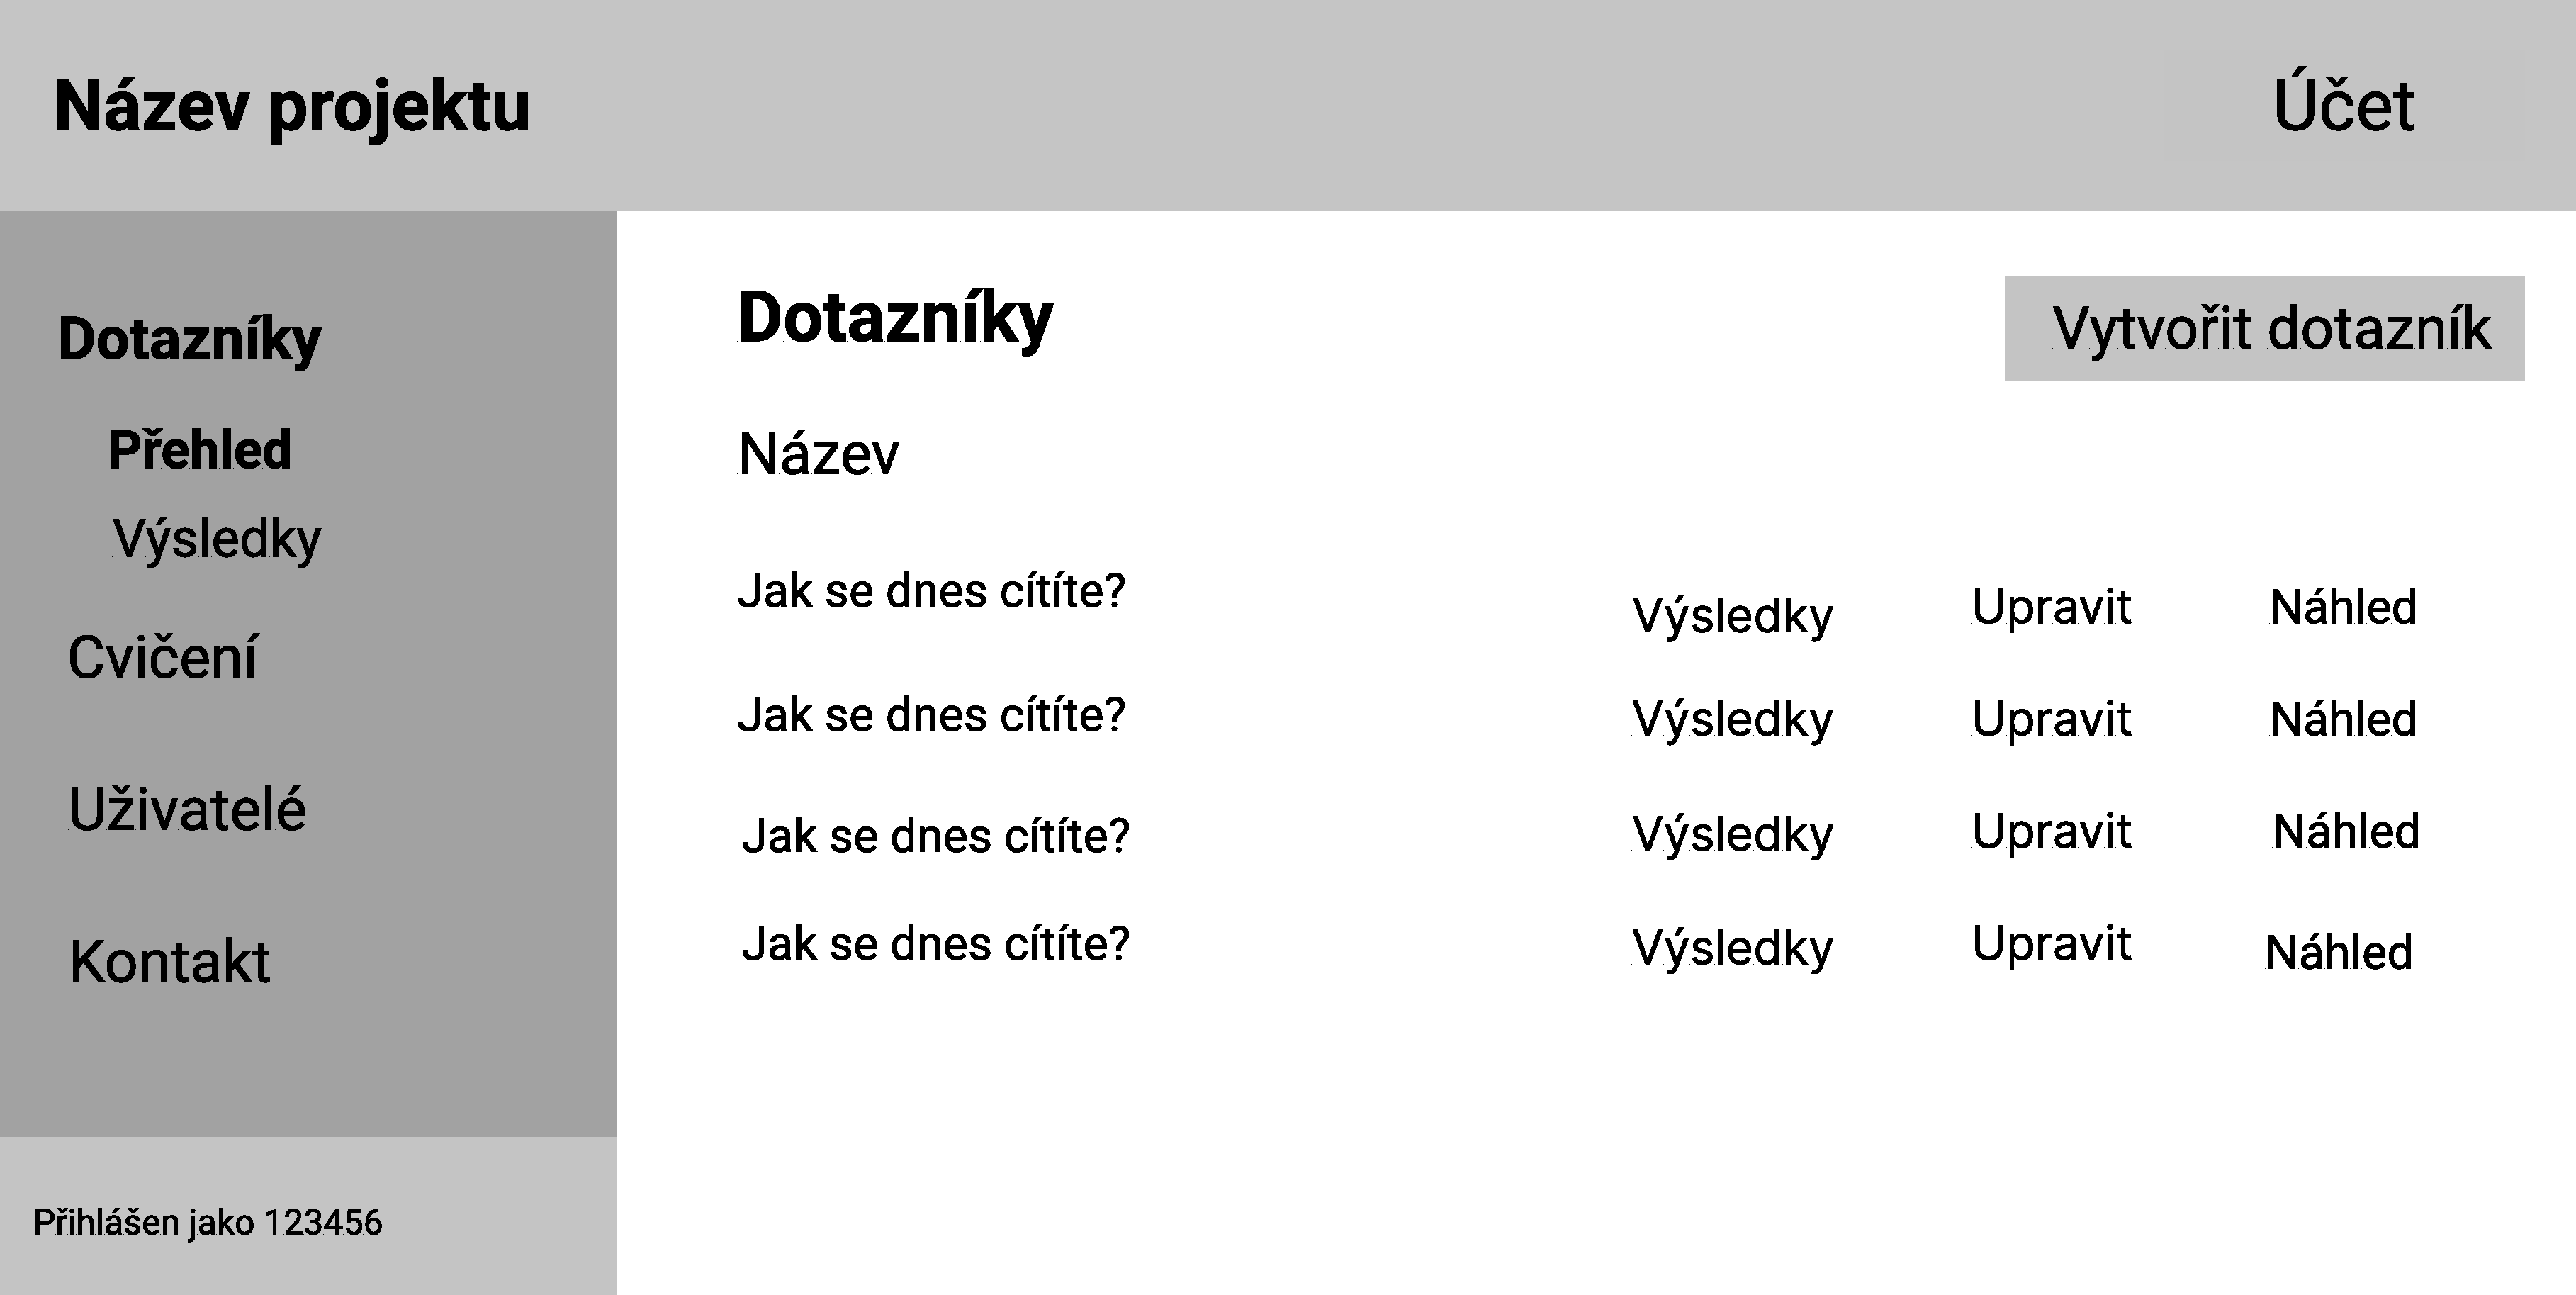
\includegraphics[width=\textwidth]{../attachments/design/zamestnanec/dotazniky-prehled}
    \caption{Přehledová stránka pro definice dotazníků pro zaměstnance}\label{fig:prehled-zamestnanec}
\end{figure}

\begin{figure}[H]
    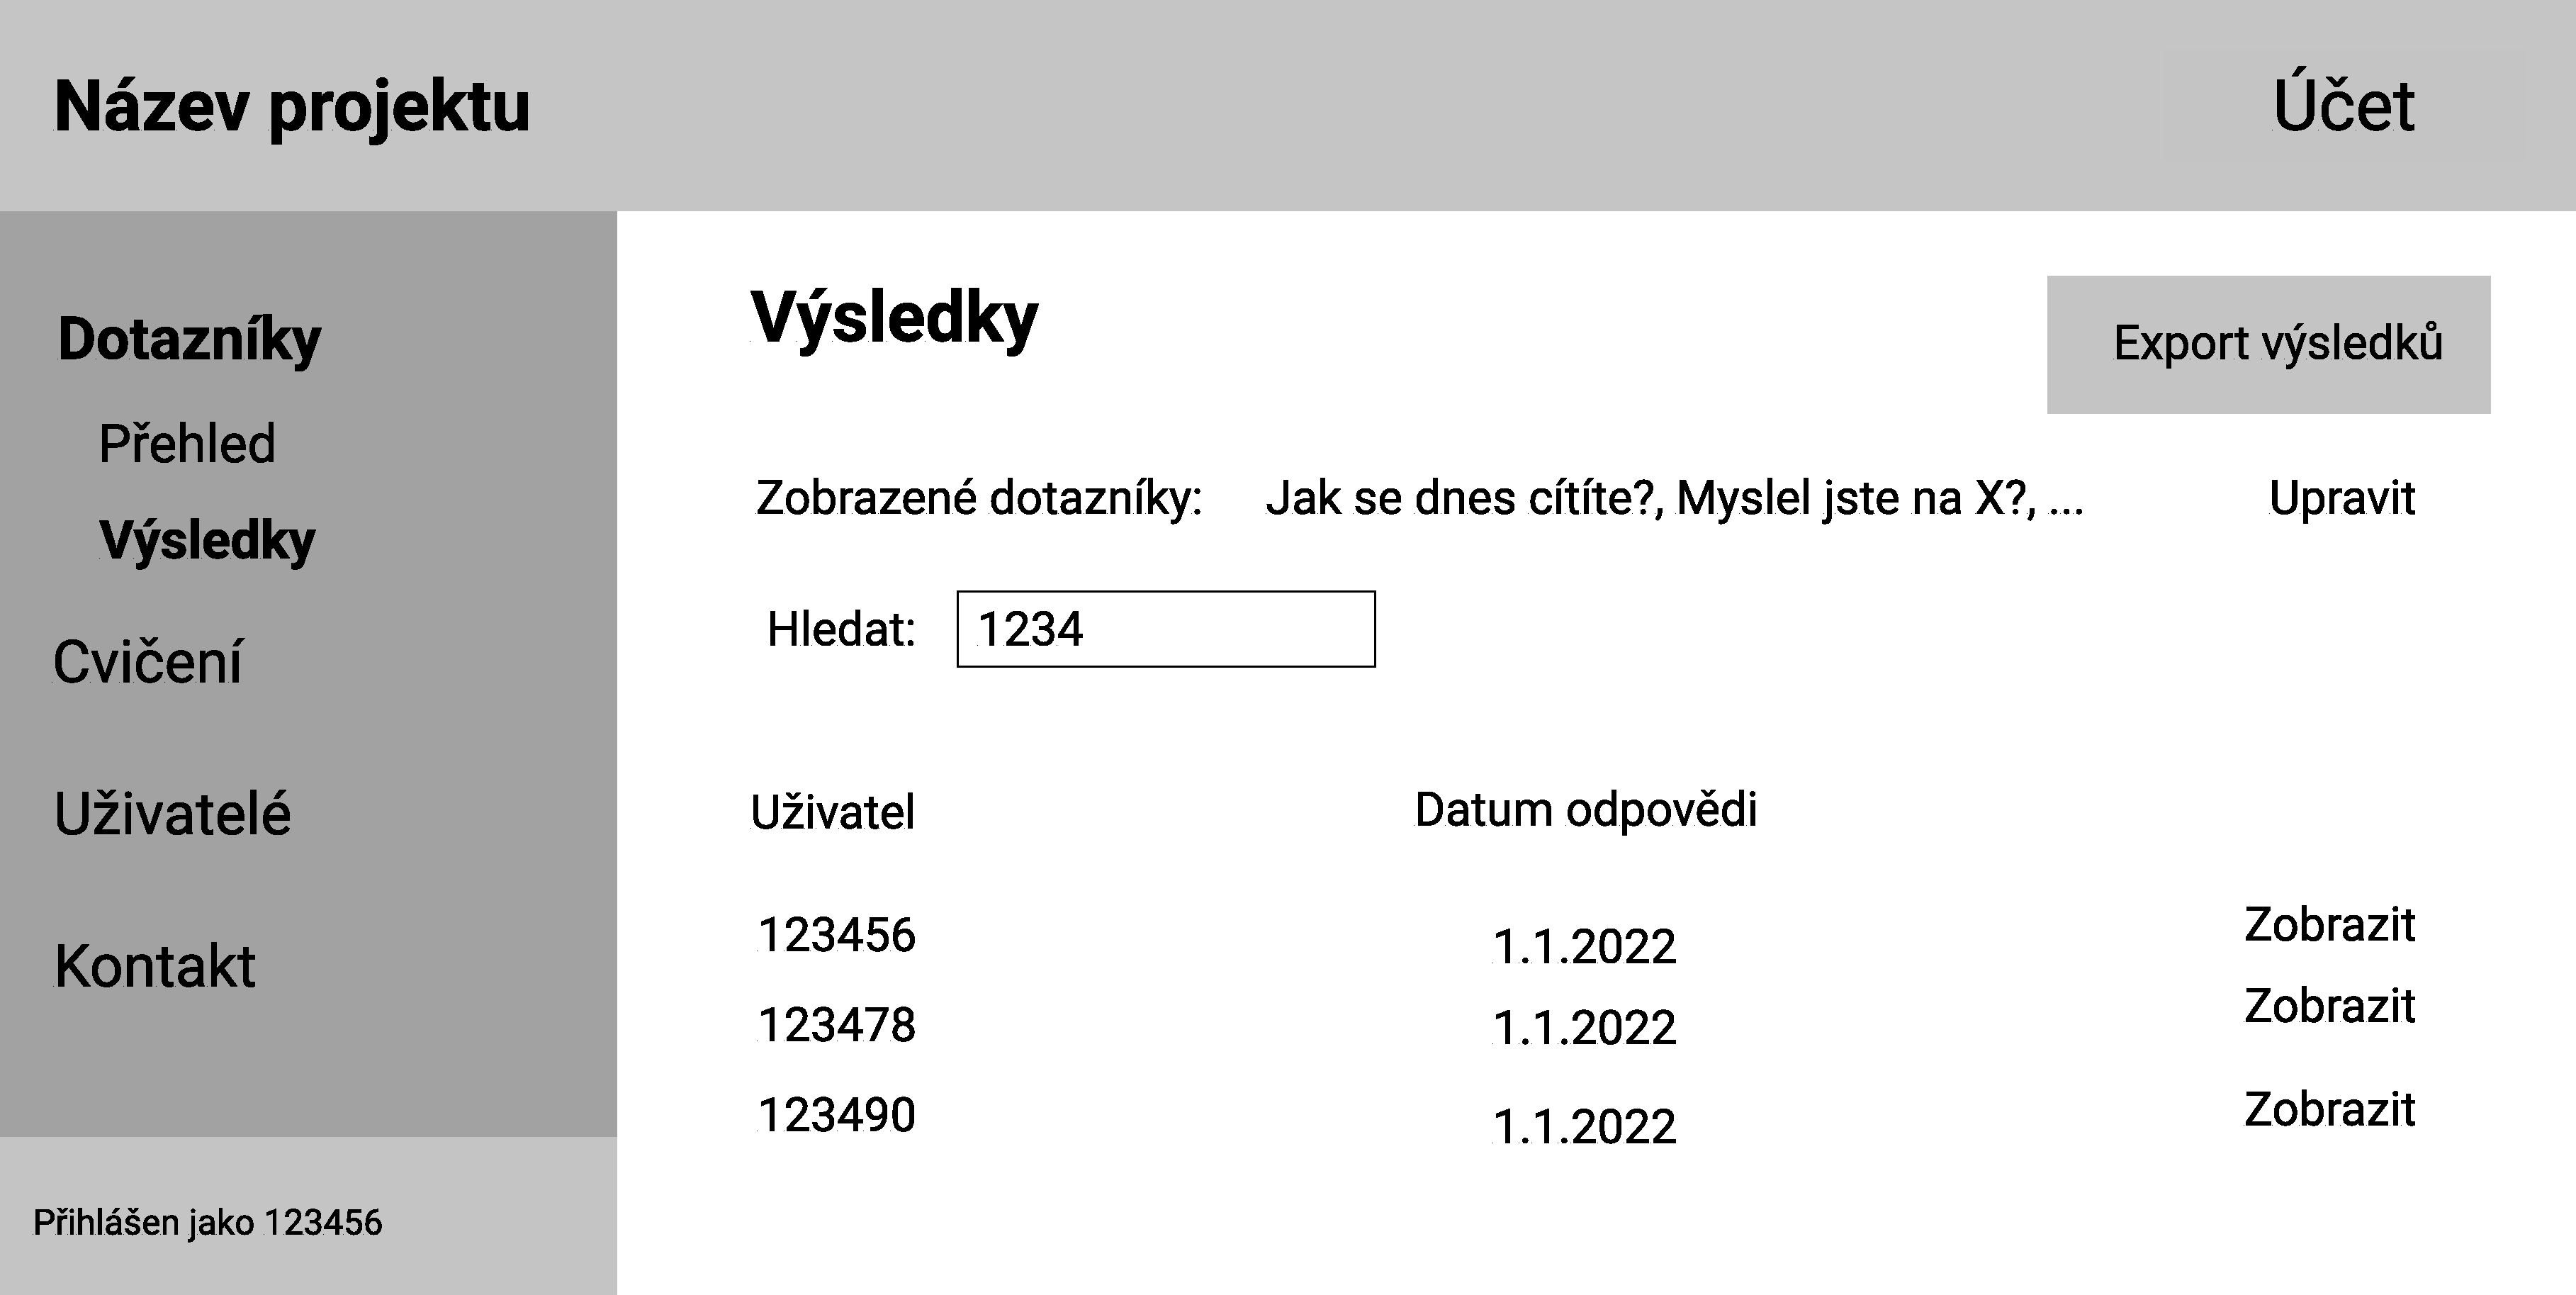
\includegraphics[width=\textwidth]{../attachments/design/zamestnanec/dotazniky-vysledky}
    \caption{Stránka s výsledky dotazníků pro zaměstnance}\label{fig:vysledky-zamestnanec}
\end{figure}

\begin{figure}[H]
    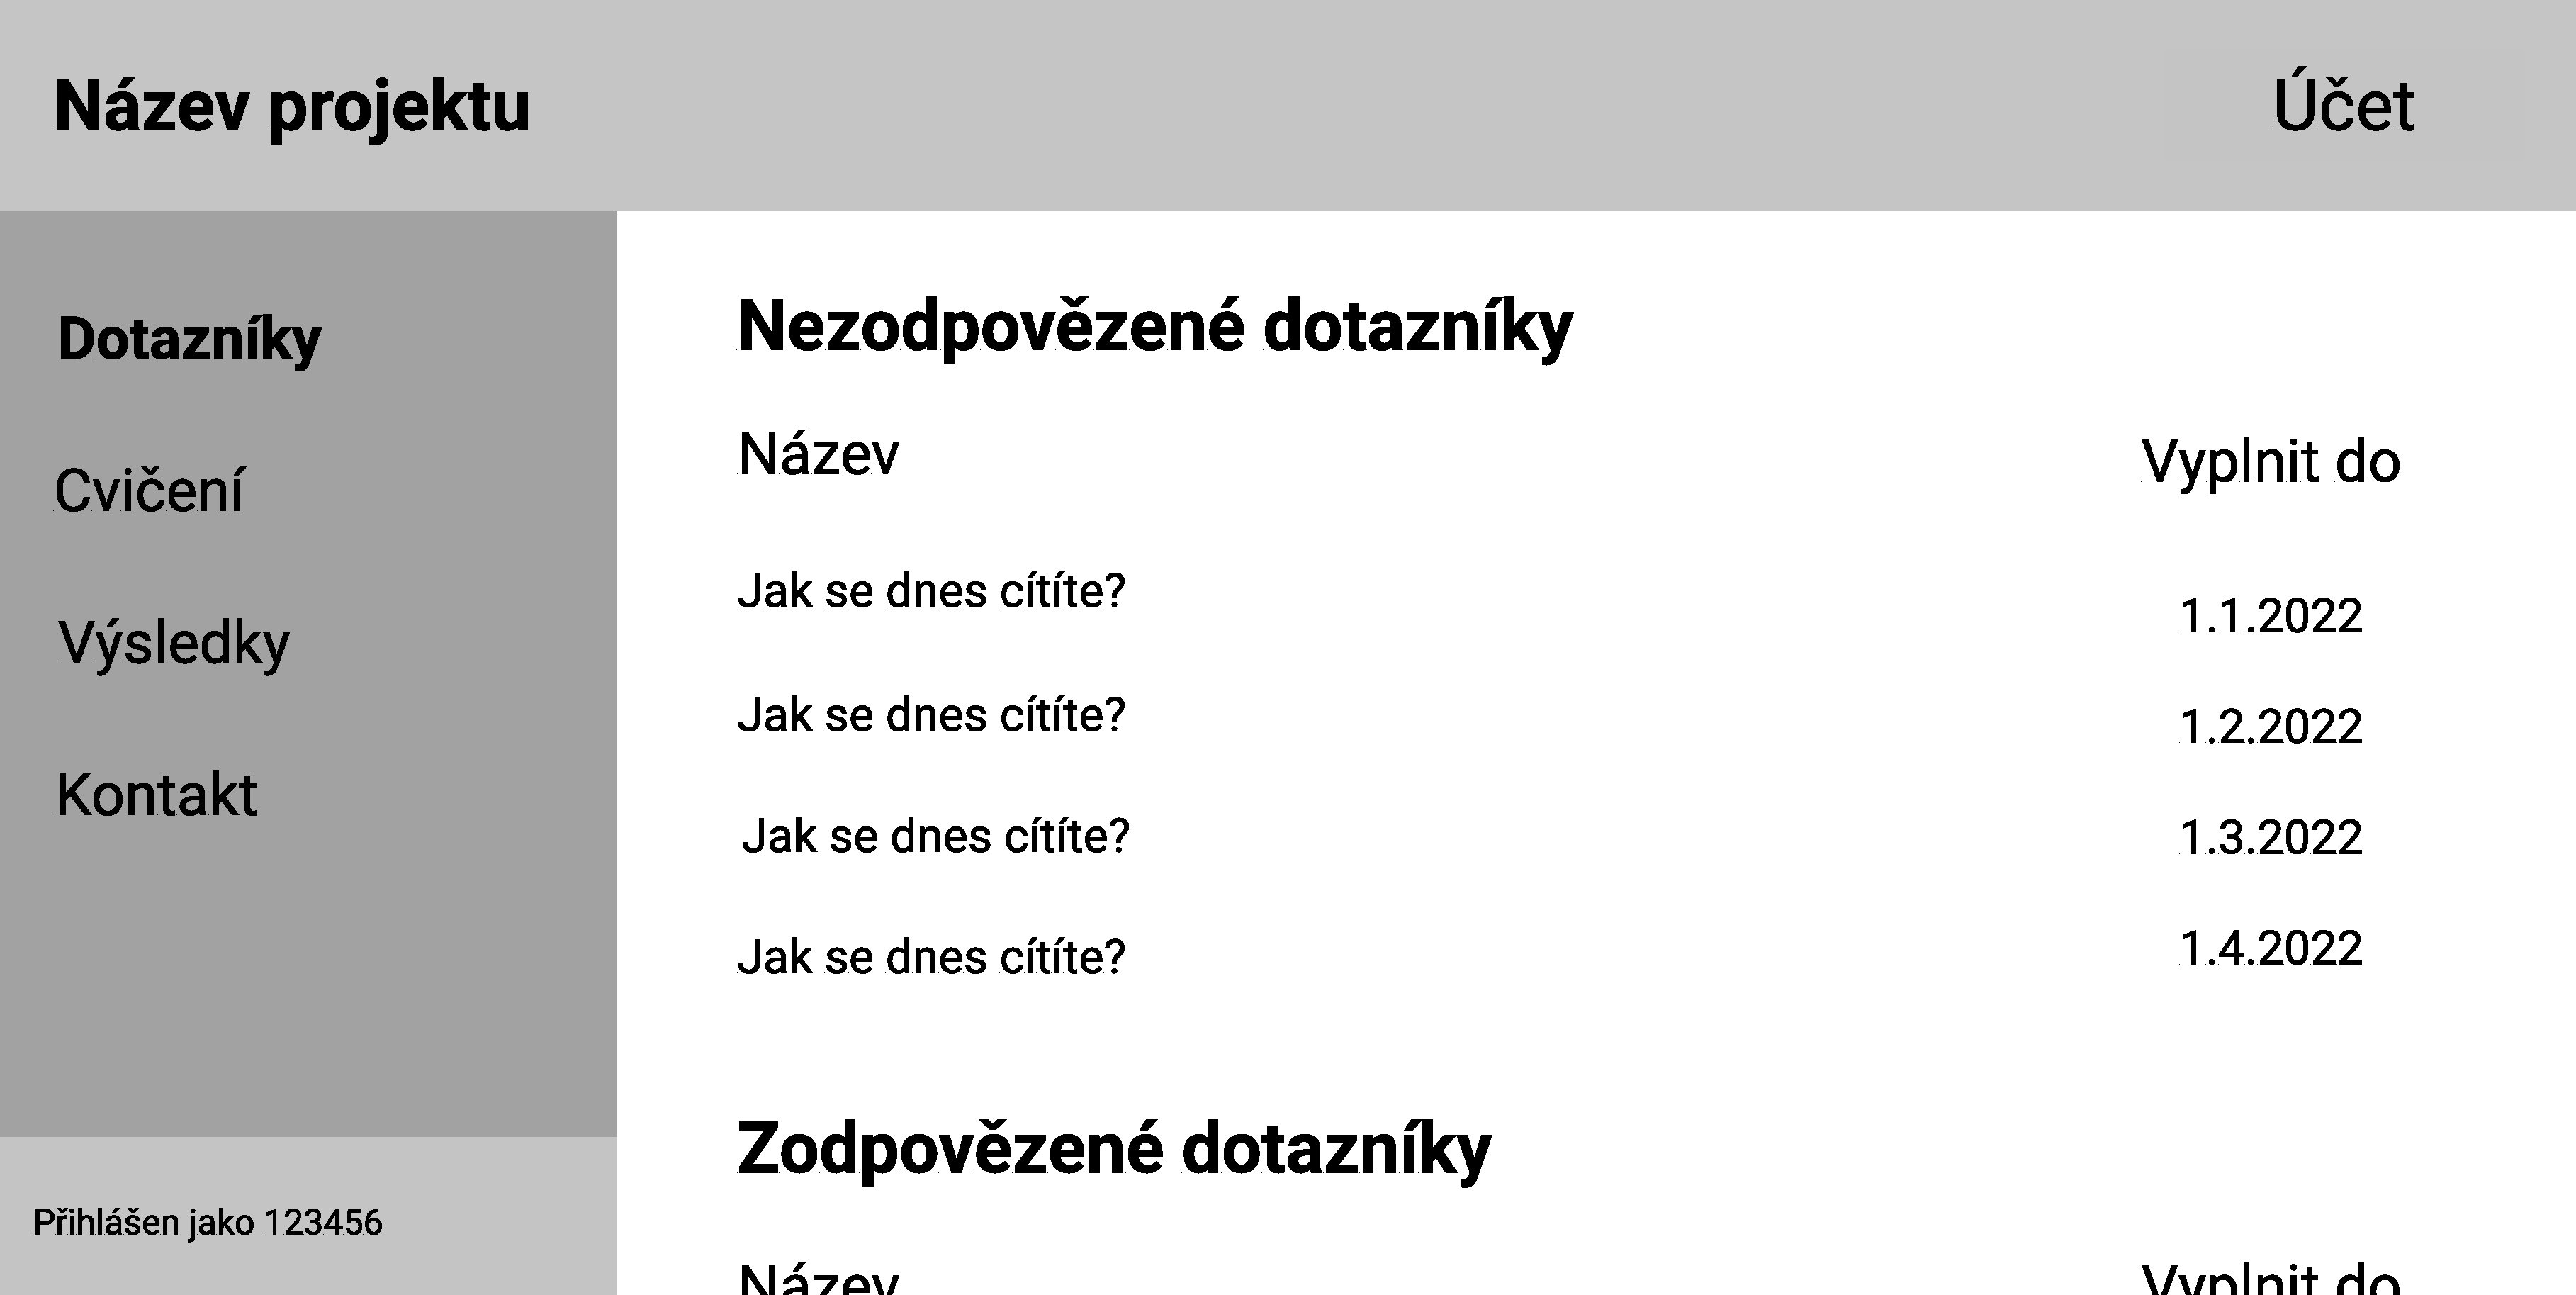
\includegraphics[width=\textwidth]{../attachments/design/uzivatel/ukoly-prehled}
    \caption{Stránka s úkoly pro uživatele}\label{fig:ukoly-prehled}
\end{figure}

\openright
\end{document}
